\documentclass[11pt,a4paper]{article}
\usepackage{fontspec}
\setmainfont{DejaVu Serif}
\setsansfont{DejaVu Sans}
\setmonofont{DejaVu Sans Mono}
\usepackage{polyglossia}
\setdefaultlanguage[script=latin]{serbian}
\usepackage[a4paper,top=2.4cm,bottom=2.4cm,left=2.6cm,right=2.4cm]{geometry}
\usepackage{setspace}
\setstretch{1.18}
\usepackage{microtype}
\usepackage{graphicx}
% Paths are relative to this source file, so editor and command-line builds agree.
\graphicspath{{figures/}{figures_cv/}{../docs/assets/}}
\usepackage{booktabs}
\usepackage{tabularx}
\usepackage{array}
\usepackage{multirow}
\usepackage{float}
\usepackage{caption}
\usepackage{amsmath,amssymb}
\usepackage{siunitx}
\sisetup{output-decimal-marker={,},group-separator={\,},group-minimum-digits=4}
\usepackage{xcolor}
\definecolor{etfblue}{RGB}{31,78,121}
\definecolor{lightblue}{RGB}{220,230,241}
\definecolor{softgray}{RGB}{245,246,248}
\definecolor{encoderfill}{RGB}{222,235,247}
\definecolor{decoderfill}{RGB}{252,228,205}
\definecolor{decoderline}{RGB}{196,91,33}
\definecolor{skipgreen}{RGB}{46,125,50}
\definecolor{bottleneckfill}{RGB}{91,122,156}
\usepackage{tikz}
\usetikzlibrary{arrows.meta,positioning,shapes.geometric,fit}
\usepackage{enumitem}
\usepackage{url}
\usepackage[hidelinks,unicode]{hyperref}
\hypersetup{pdftitle={Segmentacija srčanih struktura na snimcima magnetne rezonance},pdfauthor={Vladan Bašić},pdfsubject={Projekat iz Analize biomedicinske slike}}
\captionsetup{font=small,labelfont=bf,justification=centering}
\renewcommand{\figurename}{Sl.}
\renewcommand{\tablename}{Tabela}
\renewcommand{\contentsname}{SADRŽAJ}
\setlength{\parindent}{1.25cm}
\setlength{\parskip}{0pt}
\setlength{\emergencystretch}{3em}
\setlist[itemize]{nosep,leftmargin=1.2cm}
\setcounter{tocdepth}{2}
\newcommand{\LV}{\mathrm{LV}}
\newcommand{\RV}{\mathrm{RV}}
\newcommand{\Myo}{\mathrm{Myo}}
\newcommand{\ED}{\mathrm{ED}}
\newcommand{\ES}{\mathrm{ES}}
\begin{document}
\begin{titlepage}
\thispagestyle{empty}
\noindent
\begin{minipage}[t]{0.18\textwidth}\vspace{0pt}\includegraphics[width=2.25cm]{ETFBg.png}\end{minipage}%
\begin{minipage}[t]{0.58\textwidth}\vspace{0.15cm}\centering
{\large Univerzitet u Beogradu\par}\vspace{0.12cm}{\large\bfseries Elektrotehnički fakultet\par}\vspace{0.12cm}{\normalsize Katedra za signale i sisteme\par}
\end{minipage}%
\begin{minipage}[t]{0.18\textwidth}\vspace{0.25cm}\raggedleft\includegraphics[width=2.25cm]{SIS.png}\end{minipage}
\vfill
\begin{center}
{\LARGE\bfseries DIPLOMSKI RAD\par}\vspace{0.35cm}
\vspace{1.6cm}
{\LARGE\bfseries Segmentacija srčanih struktura na snimcima magnetne rezonance:\par}\vspace{0.25cm}
{\LARGE\bfseries 2D i 3D neuronske mreže na ACDC bazi\par}
\vspace{2.0cm}{\large\bfseries Student\par}\vspace{0.12cm}{\large Vladan Bašić, 2022/0395\par}
\vspace{1.7cm}{\large\bfseries Mentor\par}\vspace{0.12cm}{\large prof. dr Milica Janković\par}
\end{center}
\vfill
\begin{center}{\large\itshape Beograd, septembar 2026. godine}\end{center}
\end{titlepage}
\setcounter{page}{2}

\section*{REZIME}
\addcontentsline{toc}{section}{REZIME}
U ovom projektu realizovan je postupak automatske segmentacije desne komore, miokarda i leve komore na kinematografskim MR snimcima srca u kratkoj osi. Postupak obuhvata konverziju NIfTI podataka u HDF5 uz očuvanje prostornog razmaka voksela i afine transformacije, resamplovanje, normalizaciju intenziteta, obuku neuronskih mreža i evaluaciju nakon rekonstrukcije celih trodimenzionih volumena. Posebna pažnja posvećena je promenljivoj i anizotropnoj rezoluciji ACDC baze.

Upoređeni su FCN-8, standardni 2D U-Net, modifikovani 2D U-Net i anizotropni 3D U-Net. Umesto jedne fiksne podele, 100 označenih trening pacijenata podeljeno je deterministički na pet dijagnostički stratifikovanih foldova. U svakom foldu obučava se na 80, a validira na 20 pacijenata; svaka od pet dijagnostičkih grupa zastupljena je sa 16/4 pacijenta. Najveći srednji volumetrijski Dice koeficijent u unakrsnoj validaciji postiže standardni 2D U-Net, $0{,}9025\pm0{,}0064$. Njegov ansambl od pet modela postiže Dice $0{,}9109$ na odvojenih 50 test pacijenata.

Metrike Dice, ASSD i Hausdorffovo rastojanje računaju se na rekonstruisanim volumenima, nakon zadržavanja najveće povezane komponente svake ciljne klase. Rastojanja se računaju sa fizičkim razmakom u milimetrima. Petostruka validacija prikazuje varijaciju rezultata između foldova, a normalizacija fizičke skale omogućava računanje rastojanja u milimetrima.
\clearpage
\tableofcontents
\clearpage

\section{UVOD}
Kardiovaskularna magnetna rezonanca (CMR) omogućava neinvazivno sagledavanje anatomije i funkcije srca. Kinematografski MR snimak obuhvata više vremenskih trenutaka tokom srčanog ciklusa, dok niz preseka u kratkoj osi pokriva srce od baze do vrha. Za kvantitativnu analizu potrebno je odrediti granice šupljina leve i desne komore i mišićnog zida leve komore. Na osnovu tih kontura izračunavaju se zapremine na kraju dijastole i sistole, udarni volumen, ejekciona frakcija i masa miokarda. Smernice za CMR analizu preporučuju izveštavanje zapremina i ejekcionih frakcija obe komore, jer su ove veličine važne za procenu srčane funkcije \cite{scmr2022}.

Leva komora (eng. \textit{left ventricle}, LV) potiskuje oksigenisanu krv u sistemsku cirkulaciju, dok desna komora (eng. \textit{right ventricle}, RV) potiskuje krv prema plućima. Miokard (Myo) predstavlja mišićni zid leve komore između endokardne i epikardne konture. Krajnja dijastola (ED) odgovara najvećoj ispunjenosti komora, a krajnja sistola (ES) njihovoj najvećoj kontrakciji. Ako su $V_{ED}$ i $V_{ES}$ zapremine komore, ejekciona frakcija iznosi
\begin{equation}
EF=\frac{V_{ED}-V_{ES}}{V_{ED}}\cdot100\,\%.
\end{equation}

Ručno iscrtavanje kontura zahteva stručnost i vreme, a rezultat može zavisiti od posmatrača. Automatska segmentacija svakom pikselu ili vokselu dodeljuje pozadinu, RV, miokard ili LV. Konvolucione neuronske mreže uče hijerarhijska obeležja direktno iz slike i pogodne su za ovu gustu višeklasnu klasifikaciju \cite{litjens2017}.

Poseban problem kod MR snimaka srca jeste anizotropija. ACDC volumeni imaju in-plane razmak približno $0{,}703$--$1{,}953$ mm, a razmak duž ose preseka $5$--$10$ mm. Zbog toga susedni vokseli nemaju isto fizičko rastojanje u svim pravcima, pa agresivna 3D obrada može izgubiti informaciju duž ose preseka. Baumgartner i saradnici pokazali su da 2D mreže mogu biti konkurentnije od 3D mreža upravo zbog malog broja preseka, niske rezolucije kroz ravan i većeg broja 2D uzoraka za obuku \cite{baumgartner2017}.

Cilj projekta je reprodukcija i proširenje tog postupka: poređenje FCN-8, standardnog i modifikovanog 2D U-Net-a i anizotropnog 3D U-Net-a, uz očuvanje prostornih metapodataka, normalizaciju fizičke skale i procenu kvaliteta na nivou celih volumena. U odnosu na raniji eksperiment sa jednom podelom, ovde se koristi deterministička dijagnostički stratifikovana petostruka validacija i odvojena evaluacija petomodelnog ansambla.

\section{METODOLOGIJA RADA}
\subsection{Baza podataka ACDC}
Automatic Cardiac Diagnosis Challenge sadrži 150 cine-CMR pregleda sa ED i ES referencama za LV, RV i miokard \cite{bernard2018,acdcweb}. Sto pacijenata 001--100 korišćeno je isključivo za obuku i unakrsnu validaciju, dok 50 pacijenata 101--150 ostaje odvojeno za završnu lokalnu evaluaciju ansambla. Dijagnoze DCM, HCM, MINF, NOR i RV ravnomerno su zastupljene.

\begin{table}[H]
\centering
\caption{Dijagnostičke grupe u ACDC bazi \cite{bernard2018}.}
\label{tab:acdc-groups}
\begin{tabularx}{\textwidth}{>{\bfseries}l l X c c}
\toprule
Oznaka & Naziv & Osnovna karakteristika & Obuka & Test \\
\midrule
NOR & normalni ispitanici & uredna funkcija i dimenzije komora & 20 & 10 \\
MINF & prethodni infarkt miokarda & snižena LV ejekciona frakcija i regionalni poremećaj kontrakcije & 20 & 10 \\
DCM & dilatativna kardiomiopatija & proširena LV šupljina i snižena ejekciona frakcija & 20 & 10 \\
HCM & hipertrofična kardiomiopatija & zadebljan miokard uz očuvanu funkciju & 20 & 10 \\
RV & abnormalna desna komora & povećana zapremina i/ili smanjena funkcija RV & 20 & 10 \\
\bottomrule
\end{tabularx}
\end{table}

\begin{figure}[H]
\centering
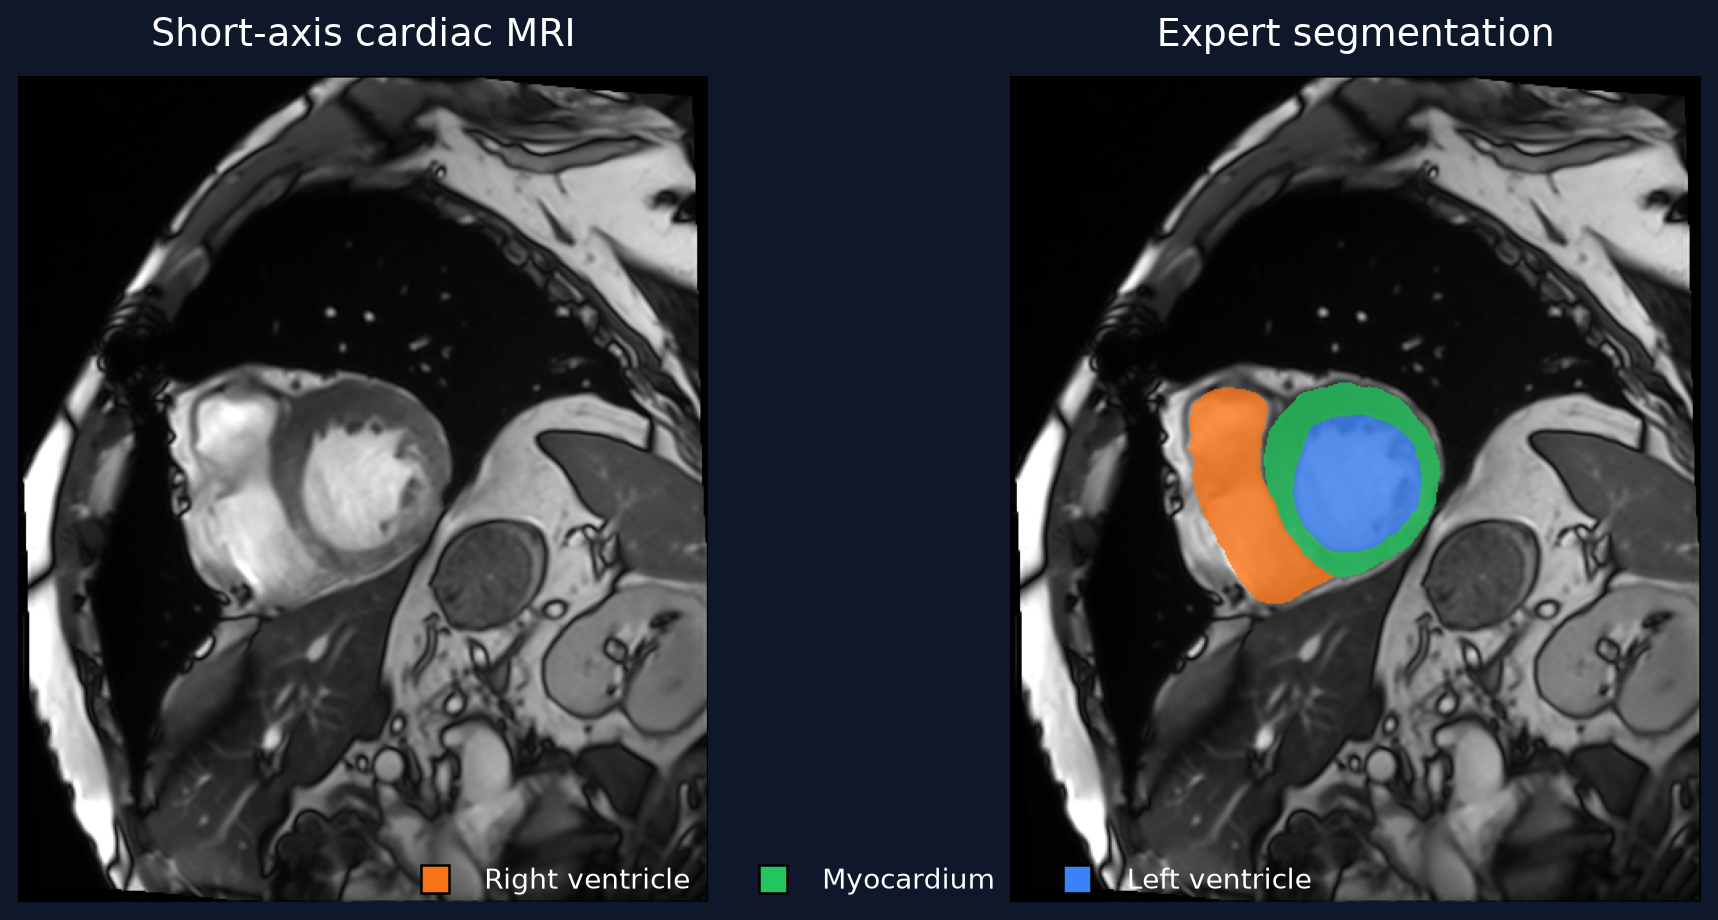
\includegraphics[width=0.93\textwidth]{acdc_segmentation_example.png}
\caption{Primer MR preseka iz ACDC baze i ekspertske segmentacije desne komore, miokarda i leve komore.}
\label{fig:dataset-example}
\end{figure}

Pacijenti se dele sa semenom 42 na pet foldova. Svaki fold ima 80 pacijenata za obuku i 20 za validaciju, pri čemu su svi preseci i obe faze jednog pacijenta u istom foldu. Time se sprečava curenje informacija između obuke i validacije i omogućava procena varijabilnosti rezultata.

\subsection{Blok dijagram sistema}
Ulazni NIfTI podaci najpre se prevode u HDF5 format uz očuvanje slike, oznake i prostornih metapodataka. Zatim se formiraju posebni 2D i 3D skupovi. U svakom foldu model vidi samo pacijente za obuku, dok se za evaluaciju čuvaju težine iz epohe sa najboljim validacionim foreground Dice rezultatom. Nakon predikcije, 2D preseci se ponovo slažu u volumene, uklanjaju se male izolovane komponente i izlaz se poredi sa ekspertskom referencom.

\subsection{Konverzija, prostorni razmak i predobrada}
NIfTI slike i maske prevode se u HDF5 uz čuvanje identifikatora pacijenta, dijagnoze, faze, oblika volumena, afine transformacije i razmaka u redosledu $Z\times Y\times X$. Uz intenzitete i oznake čuvaju se i broj vremenskog okvira i položaj preseka. Prostorni razmak koristi se za resamplovanje i računanje fizičkih rastojanja, dok identifikator pacijenta i dijagnoza određuju stratifikovanu podelu. Prostorni razmak nije dodatni ulazni kanal mreže.

\begin{figure}[H]
\centering
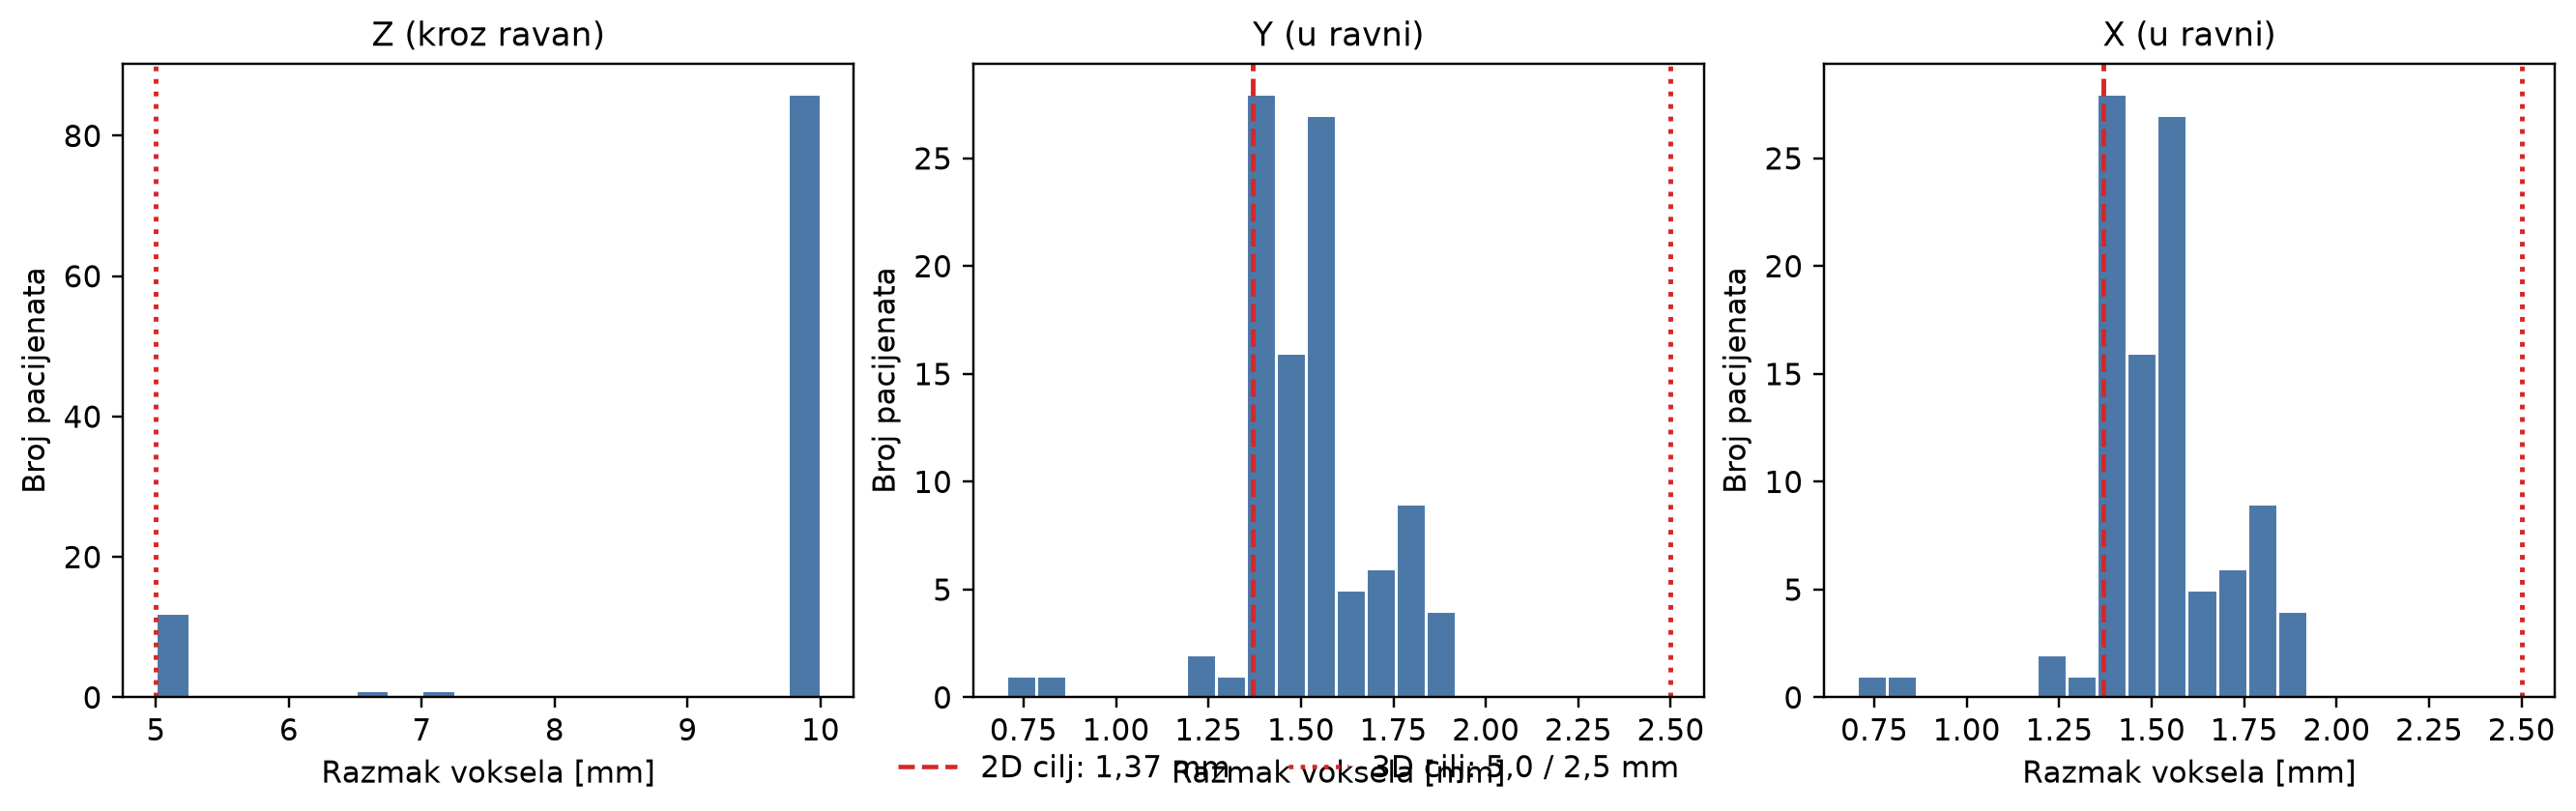
\includegraphics[width=\textwidth]{spacing_distribution.png}
\caption{Raspodela izvornog razmaka voksela trening pacijenata. Crvene linije označavaju ciljne razmake 2D i 3D predobrade.}
\label{fig:spacing}
\end{figure}

Za 2D mreže svaki presek se resampluje samo unutar ravni na $1{,}37\times1{,}37$ mm. Osa kroz preseke se ne interpolira, čime se izbegavaju artefakti pri velikom i promenljivom razmaku preseka. FCN-8 koristi $224\times224$, a oba U-Net modela $396\times396$ piksela. Za 3D model volumen se resampluje na $5{,}0\times2{,}5\times2{,}5$ mm i centralno dovodi na $60\times204\times204$ voksela. Na slikama se koristi linearna, a na maskama interpolacija najbližeg suseda. Intenziteti se standardizuju po slici, dok se preveliki ulazi centralno isecaju, a manji dopunjuju nulama.

\begin{table}[H]
\centering
\caption{Parametri predobrade po arhitekturi.}
\label{tab:preprocessing}
\begin{tabular}{lccc}
\toprule
Arhitektura & Ciljni razmak & Ulazna veličina & Jedinica obuke \\
\midrule
FCN-8 & $1{,}37\times1{,}37$ mm & $224\times224$ & 2D presek \\
2D U-Net & $1{,}37\times1{,}37$ mm & $396\times396$ & 2D presek \\
modifikovani 2D U-Net & $1{,}37\times1{,}37$ mm & $396\times396$ & 2D presek \\
modifikovani 3D U-Net & $5{,}0\times2{,}5\times2{,}5$ mm & $60\times204\times204$ & 3D volumen \\
\bottomrule
\end{tabular}
\end{table}

\begin{figure}[H]
\centering
\resizebox{0.96\textwidth}{!}{%
\begin{tikzpicture}[
node distance=8mm and 9mm,
block/.style={draw=etfblue,rounded corners,fill=lightblue,align=center,minimum height=1.05cm,text width=2.7cm,font=\small},
smallblock/.style={draw=black!55,rounded corners,fill=softgray,align=center,minimum height=0.95cm,text width=2.55cm,font=\small},
arrow/.style={-{Stealth[length=2.2mm]},thick,draw=etfblue}]
\node[block] (nifti) {ACDC NIfTI\\slike i maske};
\node[block,right=of nifti] (hdf5) {HDF5 konverzija\\i metapodaci};
\node[smallblock,above right=7mm and 10mm of hdf5] (prep2) {2D predobrada\\$224^2$ / $396^2$};
\node[smallblock,below right=7mm and 10mm of hdf5] (prep3) {3D predobrada\\$60\times204\times204$};
\node[smallblock,right=of prep2] (models2) {FCN-8 i 2D\\U-Net modeli};
\node[smallblock,right=of prep3] (models3) {anizotropni\\3D U-Net};
\node[block,right=18mm of models2,yshift=-14mm] (volume) {rekonstrukcija volumena\\i najveće komponente};
\node[block,right=of volume] (metrics) {Dice, ASSD, HD\\i analiza rezultata};
\draw[arrow] (nifti)--(hdf5); \draw[arrow] (hdf5)--(prep2); \draw[arrow] (hdf5)--(prep3);
\draw[arrow] (prep2)--(models2); \draw[arrow] (prep3)--(models3);
\draw[arrow] (models2)--(volume); \draw[arrow] (models3)--(volume); \draw[arrow] (volume)--(metrics);
\end{tikzpicture}}
\caption{Blok dijagram spacing-aware sistema za segmentaciju.}
\label{fig:pipeline}
\end{figure}

\subsection{Arhitekture neuronskih mreža}
\subsubsection{FCN-8}
Potpuno konvoluciona mreža zamenjuje potpuno povezane slojeve klasifikacione mreže konvolucijama i time omogućava gustu predikciju klase za svaki piksel \cite{long2015}. Ulaz FCN-8 je jedan standardizovan MR presek veličine $224\times224$. Enkoder ima pet VGG-stil blokova širina 64, 128, 256, 512 i 512 kanala; prva dva bloka sadrže po dve, a naredna tri po tri konvolucije $3\times3$ sa dopunom jedan. Iza svakog bloka sledi maksimalno sažimanje $2\times2$ sa korakom dva, pa prostorna rezolucija redom prelazi sa $224$ na 112, 56, 28, 14 i 7 piksela.

Klasifikaciona glava na mapi $7\times7$ koristi konvoluciju $7\times7$ sa 1024 kanala, ReLU i dropout 0,5, zatim konvoluciju $1\times1$ sa 1024 kanala, ReLU i dropout 0,5, a na kraju konvoluciju $1\times1$ sa četiri logita. Dve bočne grane pretvaraju izlaze pool3 (256 kanala, $28\times28$) i pool4 (512 kanala, $14\times14$) u četiri logita konvolucijom $1\times1$. Duboki rezultat se transponovanom konvolucijom $4\times4$, koraka dva, dovodi na nivo pool4 i sabira sa njegovim skorom; isti postupak se ponavlja do pool3. Završna transponovana konvolucija $16\times16$, koraka osam, vraća četiri logita na izvornu rezoluciju. Sve obične konvolucije koriste batch normalizaciju i ReLU; transponovane konvolucije se inicijalizuju bilinearnim filtrom. Ukupno se optimizuje \num{41474508} parametara.

\begin{figure}[H]
\centering
\resizebox{\textwidth}{!}{%
\begin{tikzpicture}[
feature/.style={draw=etfblue,very thick,rounded corners=2pt,fill=encoderfill,align=center,minimum height=13mm,text width=20mm,font=\scriptsize},
input/.style={draw=black!55,rounded corners=2pt,fill=softgray,align=center,minimum height=13mm,text width=17mm,font=\scriptsize},
head/.style={draw=decoderline,very thick,rounded corners=2pt,fill=decoderfill,align=center,minimum height=13mm,text width=25mm,font=\scriptsize},
fusion/.style={draw=decoderline,rounded corners=2pt,fill=decoderfill,align=center,minimum height=10mm,text width=19mm,font=\scriptsize},
sum/.style={circle,draw=decoderline,very thick,fill=white,inner sep=0pt,minimum size=5mm,font=\bfseries\small},
encarrow/.style={-{Stealth[length=2mm]},thick,draw=etfblue},
decarr/.style={-{Stealth[length=2mm]},very thick,draw=decoderline},
skip/.style={-{Stealth[length=1.8mm]},draw=skipgreen,dashed,very thick},
lab/.style={font=\tiny,fill=white,inner sep=1pt}]
\node[input]   (in) at (0,2.7) {MR presek\\$1\times224^2$};
\node[feature] (b1) at (2.2,2.7) {blok 1 + pool1\\$2\times\mathrm{Conv}_{3^2}$\\$64\times112^2$};
\node[feature] (b2) at (4.5,2.7) {blok 2 + pool2\\$2\times\mathrm{Conv}_{3^2}$\\$128\times56^2$};
\node[feature] (b3) at (6.8,2.7) {blok 3 + pool3\\$3\times\mathrm{Conv}_{3^2}$\\$256\times28^2$};
\node[feature] (b4) at (9.1,2.7) {blok 4 + pool4\\$3\times\mathrm{Conv}_{3^2}$\\$512\times14^2$};
\node[feature] (b5) at (11.4,2.7) {blok 5 + pool5\\$3\times\mathrm{Conv}_{3^2}$\\$512\times7^2$};
\node[head]    (head) at (14.0,2.7) {klasifikaciona glava\\$7^2\!:\,512\rightarrow1024$\\$1^2\!:\,1024\rightarrow1024\rightarrow4$};
\node[sum] (add4) at (11.5,0) {$+$};
\node[fusion] (f4) at (9.8,0) {spojeni skor\\$4\times14^2$};
\node[sum] (add3) at (7.5,0) {$+$};
\node[fusion] (f3) at (5.8,0) {spojeni skor\\$4\times28^2$};
\node[head] (out) at (2.7,0) {segmentacioni logiti\\$4\times224^2$};
\draw[encarrow] (in)--(b1); \draw[encarrow] (b1)--(b2); \draw[encarrow] (b2)--(b3);
\draw[encarrow] (b3)--(b4); \draw[encarrow] (b4)--(b5); \draw[encarrow] (b5)--(head);
\draw[decarr] (head.south) |- node[lab,pos=.72] {$\mathrm{TConv}_{4^2},\ s=2$} (add4.east);
\draw[skip] (b4.south) -- node[lab,right] {$\mathrm{Conv}_{1^2}:512\rightarrow4$} (add4.north);
\draw[decarr] (add4)--(f4);
\draw[decarr] (f4)-- node[lab] {$\mathrm{TConv}_{4^2},\ s=2$} (add3);
\draw[skip] (b3.south) -- node[lab,right] {$\mathrm{Conv}_{1^2}:256\rightarrow4$} (add3.north);
\draw[decarr] (add3)--(f3);
\draw[decarr] (f3)-- node[lab] {$\mathrm{TConv}_{16^2},\ s=8$} (out);
\node[font=\scriptsize,text=etfblue] at (6.8,3.65) {VGG-stil enkoder: smanjivanje prostorne rezolucije};
\node[font=\scriptsize,text=decoderline] at (8.8,-0.85) {dekoder skorova: nadodabiranje i sabiranje};
\end{tikzpicture}}
\caption{Šema arhitekture FCN-8. Plava putanja izdvaja obeležja, narandžasta vraća prostornu rezoluciju, a zelene isprekidane grane projektuju pool3 i pool4 mape na četiri klasna skora. Krugovi označavaju sabiranje, ne nadovezivanje kanala.}
\label{fig:fcn8-architecture}
\end{figure}

\subsubsection{Standardni i modifikovani 2D U-Net}
U-Net ima kontrakcionu putanju za izdvajanje konteksta i simetričnu ekspanzionu putanju za preciznu lokalizaciju \cite{ronneberger2015}. Standardni 2D model prima $1\times396\times396$ i koristi osnovnu širinu 64. Enkoder se sastoji od četiri bloka sa po dve konvolucije $3\times3$, batch normalizacijom i ReLU aktivacijom, sa 64, 128, 256 i 512 kanala. Maksimalna sažimanja $2\times2$ daju mape dimenzija $396$, 198, 99 i 49, a nakon četvrtog sažimanja usko grlo sa 1024 kanala radi na $24\times24$. Neparne dimenzije 99 i 49 potiču od ulaza 396; pri dekodovanju se, kada je potrebno, mapa bilinearnom interpolacijom usklađuje sa dimenzijom preskočne grane.

Dekoder ima četiri nivoa. Na svakom se transponovanom konvolucijom $2\times2$, koraka dva, prepolovi broj kanala (1024--512--256--128--64), rezultat se nadovezuje sa odgovarajućom enkoderskom mapom, pa dve konvolucije $3\times3$ obrađuju spojene kanale. Završna konvolucija $1\times1$ preslikava 64 kanala u četiri logita: pozadinu, RV, Myo i LV. Standardni 2D U-Net ima \num{31044484} parametara.

Modifikovani 2D U-Net ima potpuno isti ulaz, enkoder, usko grlo i izlazne širine dekoderskih blokova. Razlika je samo u svakoj od četiri transponovane konvolucije: umesto 512, 256, 128 i 64 kanala, one daju četiri kanala, koliko postoji klasa. Posle nadovezivanja širine spojenih mapa su 516, 260, 132 i 68 kanala, a naredni par konvolucija ih ponovo svodi na 512, 256, 128 i 64. Tako se sužava najskuplji deo dekoderske putanje bez promene izlazne rezolucije. Model ima \num{25188212} parametara, \(\num{5856272}\) manje od standardnog 2D U-Net-a, odnosno približno 18,9\% manje.

\begin{figure}[H]
\centering
\resizebox{\textwidth}{!}{%
\begin{tikzpicture}[
enc/.style={draw=etfblue,very thick,rounded corners=2pt,fill=encoderfill,align=center,minimum height=14mm,text width=22mm,font=\scriptsize},
dec/.style={draw=decoderline,very thick,rounded corners=2pt,fill=decoderfill,align=center,minimum height=18mm,text width=25mm,font=\scriptsize},
bneck/.style={draw=etfblue,very thick,rounded corners=2pt,fill=bottleneckfill,text=white,align=center,minimum height=14mm,text width=22mm,font=\scriptsize},
output/.style={draw=black!55,rounded corners=2pt,fill=softgray,align=center,minimum height=12mm,text width=23mm,font=\scriptsize},
down/.style={-{Stealth[length=2mm]},thick,draw=etfblue},
up/.style={-{Stealth[length=2mm]},very thick,draw=decoderline},
skip/.style={-{Stealth[length=1.8mm]},draw=skipgreen,dashed,very thick},
op/.style={font=\tiny,fill=white,inner sep=1pt,align=center}]
\node[enc] (e1) at (0,3.2) {enkoder 1\\$64\times396^2$};
\node[enc] (e2) at (2.8,3.2) {enkoder 2\\$128\times198^2$};
\node[enc] (e3) at (5.6,3.2) {enkoder 3\\$256\times99^2$};
\node[enc] (e4) at (8.4,3.2) {enkoder 4\\$512\times49^2$};
\node[bneck] (bn) at (11.2,3.2) {usko grlo\\$1024\times24^2$};
\node[dec] (d4) at (8.4,0) {dekoder 4\\std. $512\rightarrow1024$\\mod. $4\rightarrow516$\\izlaz: $512\times49^2$};
\node[dec] (d3) at (5.6,0) {dekoder 3\\std. $256\rightarrow512$\\mod. $4\rightarrow260$\\izlaz: $256\times99^2$};
\node[dec] (d2) at (2.8,0) {dekoder 2\\std. $128\rightarrow256$\\mod. $4\rightarrow132$\\izlaz: $128\times198^2$};
\node[dec] (d1) at (0,0) {dekoder 1\\std. $64\rightarrow128$\\mod. $4\rightarrow68$\\izlaz: $64\times396^2$};
\node[output] (out) at (-2.9,0) {klasni logiti\\$\mathrm{Conv}_{1^2}$\\$4\times396^2$};
\draw[down] (e1)--node[op]{pool $2^2$}(e2);
\draw[down] (e2)--node[op]{pool $2^2$}(e3);
\draw[down] (e3)--node[op]{pool $2^2$}(e4);
\draw[down] (e4)--node[op]{pool $2^2$}(bn);
\draw[up] (bn)--(d4);
\draw[up] (d4)--(d3);
\draw[up] (d3)--(d2);
\draw[up] (d2)--(d1);
\draw[up] (d1)--(out);
\draw[skip] (e4)--(d4);
\draw[skip] (e3)--(d3); \draw[skip] (e2)--(d2); \draw[skip] (e1)--(d1);
\node[font=\scriptsize,text=etfblue] at (5.6,4.15) {kontrakciona putanja};
\node[font=\scriptsize,text=decoderline] at (4.2,-1.15) {ekspanziona putanja};
\node[draw=black!35,rounded corners,fill=white,align=left,font=\scriptsize,anchor=west,inner sep=3pt]
  at (10.0,0) {std. -- standardni U-Net\\mod. -- modifikovani U-Net\\brojevi: TConv $\rightarrow$ spoj\\blok: $2\times(\mathrm{Conv}_{3^2}+\mathrm{BN}+\mathrm{ReLU})$};
\end{tikzpicture}}
\caption{Zajednička šema standardnog i modifikovanog 2D U-Net-a. U oznakama std. i mod. par vrednosti predstavlja broj kanala posle transponovane konvolucije i posle nadovezivanja; izlaz bloka isti je u obe varijante.}
\label{fig:unet2d-architecture}
\end{figure}

\subsubsection{Anizotropni 3D U-Net}
3D U-Net koristi volumetrijske operacije i neposredno uzima u obzir kontekst susednih preseka \cite{cicek2016}. Ulaz je jedan resamplovan i dopunjen volumen $1\times60\times204\times204$ u poretku kanali$\times Z\times Y\times X$. Osnovna širina je 16, pa četiri enkoderska bloka sa po dve konvolucije $3\times3\times3$, batch normalizacijom i ReLU aktivacijom daju 16, 32, 64 i 128 kanala. Usko grlo ima 256 kanala. Standardno sažimanje faktorom dva po svim osama brzo bi uklonilo malobrojne preseke ACDC volumena; zato je samo prvo maksimalno sažimanje $(2,2,2)$, dok naredna tri imaju jezgro i korak $(1,2,2)$.

Tako se dimenzija kroz ravan menja $60\rightarrow30\rightarrow30\rightarrow30\rightarrow30$, dok dimenzije u ravni prolaze kroz $204\rightarrow102\rightarrow51\rightarrow25\rightarrow12$. Dekoder je ogledalan: prve tri transponovane konvolucije imaju korak $(1,2,2)$, a poslednja $(2,2,2)$, uz preskočne veze i dve konvolucije po nivou. Kada deljenje neparne dimenzije da 25 odnosno 51, trilinearna interpolacija usklađuje izlaz dekonvolucije sa enkoderskom mapom pre nadovezivanja. Konvolucija $1\times1\times1$ preslikava završnih 16 kanala u četiri klase. Model ima \num{5476356} parametara; to je znatno manje od 2D varijanti, ali trodimenzionalne aktivacije pri volumenu $60\times204\times204$ objašnjavaju mini-grupu veličine jedan i veći memorijski zahtev.

\begin{figure}[H]
\centering
\resizebox{\textwidth}{!}{%
\begin{tikzpicture}[
enc/.style={draw=etfblue,very thick,rounded corners=2pt,fill=encoderfill,align=center,minimum height=15mm,text width=25mm,font=\scriptsize},
dec/.style={draw=decoderline,very thick,rounded corners=2pt,fill=decoderfill,align=center,minimum height=18mm,text width=25mm,font=\scriptsize},
bneck/.style={draw=etfblue,very thick,rounded corners=2pt,fill=bottleneckfill,text=white,align=center,minimum height=15mm,text width=25mm,font=\scriptsize},
output/.style={draw=black!55,rounded corners=2pt,fill=softgray,align=center,minimum height=13mm,text width=27mm,font=\scriptsize},
down/.style={-{Stealth[length=2mm]},thick,draw=etfblue},
up/.style={-{Stealth[length=2mm]},very thick,draw=decoderline},
skip/.style={-{Stealth[length=1.8mm]},draw=skipgreen,dashed,very thick},
op/.style={font=\tiny,fill=white,inner sep=1pt,align=center}]
\node[enc] (e1) at (0,3.3) {enkoder 1\\$16\times60\times204^2$};
\node[enc] (e2) at (3.1,3.3) {enkoder 2\\$32\times30\times102^2$};
\node[enc] (e3) at (6.2,3.3) {enkoder 3\\$64\times30\times51^2$};
\node[enc] (e4) at (9.3,3.3) {enkoder 4\\$128\times30\times25^2$};
\node[bneck] (bn) at (12.4,3.3) {usko grlo\\$256\times30\times12^2$};
\node[dec] (d4) at (9.3,0) {dekoder 4\\TConv $(1,2,2)$\\$128\times30\times25^2$};
\node[dec] (d3) at (6.2,0) {dekoder 3\\TConv $(1,2,2)$\\$64\times30\times51^2$};
\node[dec] (d2) at (3.1,0) {dekoder 2\\TConv $(1,2,2)$\\$32\times30\times102^2$};
\node[dec] (d1) at (0,0) {dekoder 1\\TConv $\mathbf{(2,2,2)}$\\$16\times60\times204^2$};
\node[output] (out) at (-3.2,0) {klasni logiti\\$\mathrm{Conv}_{1^3}$\\$4\times60\times204^2$};
\draw[down] (e1)--node[op]{pool\\$\mathbf{(2,2,2)}$}(e2);
\draw[down] (e2)--node[op]{pool\\$(1,2,2)$}(e3);
\draw[down] (e3)--node[op]{pool\\$(1,2,2)$}(e4);
\draw[down] (e4)--node[op]{pool\\$(1,2,2)$}(bn);
\draw[up] (bn)--(d4);
\draw[up] (d4)--(d3);
\draw[up] (d3)--(d2);
\draw[up] (d2)--(d1);
\draw[up] (d1)--(out);
\draw[skip] (e4)--(d4);
\draw[skip] (e3)--(d3); \draw[skip] (e2)--(d2); \draw[skip] (e1)--(d1);
\node[font=\scriptsize,text=etfblue] at (6.2,4.3) {enkoder: $C\times Z\times Y\times X$};
\node[font=\scriptsize,text=decoderline] at (4.7,-1.05) {dekoder: anizotropno nadodabiranje};
\node[draw=skipgreen,rounded corners,fill=white,align=left,font=\scriptsize,anchor=west,inner sep=3pt]
  at (11.0,0) {$Z$: $60\rightarrow30\rightarrow30\rightarrow30\rightarrow30$\\$Y,X$: $204\rightarrow102\rightarrow51\rightarrow25\rightarrow12$\\\\svaki blok:\\$2\times(\mathrm{Conv}_{3^3}+\mathrm{BN}+\mathrm{ReLU})$};
\end{tikzpicture}}
\caption{Šema anizotropnog 3D U-Net-a. Podebljani koraci $(2,2,2)$ označavaju jedino sažimanje i odgovarajuće nadodabiranje duž ose preseka $Z$; na ostalim nivoima menja se samo rezolucija u ravni. Zelene isprekidane veze nadovezuju enkoderske mape na dekoderske.}
\label{fig:unet3d-architecture}
\end{figure}

\begin{table}[H]
\centering
\caption{Parametri realizovanih mreža. BN označava batch normalizaciju, a $s$ korak.}
\label{tab:architectures}
\small
\begin{tabularx}{\textwidth}{l X r}
\toprule
Model & Sastav i ključni hiperparametri & Broj parametara \\
\midrule
FCN-8 & Ulaz $1\times224^2$; VGG blokovi 64--128--256--512--512; 2/2/3/3/3 konv. $3^2$; glava 1024--1024--4, dropout 0,5; pool $2^2$, preskočne veze pool3/pool4 & \num{41474508} \\
2D U-Net & Ulaz $1\times396^2$; kanali 64--128--256--512--1024; dva $3^2$+BN+ReLU po bloku; pool/dekonv. $2^2$, $s=2$; nadovezivanje preskočnih veza & \num{31044484} \\
modifikovani 2D U-Net & Kao 2D U-Net, ali sve četiri dekonvolucije imaju izlaz od 4 kanala; dekoderski blokovi posle nadovezivanja ostaju 512--256--128--64 & \num{25188212} \\
anizotropni 3D U-Net & Ulaz $1\times60\times204^2$; kanali 16--32--64--128--256; dva $3^3$+BN+ReLU po bloku; pool/dekonv. $(2,2,2)$ jednom, zatim $(1,2,2)$ & \num{5476356} \\
\bottomrule
\end{tabularx}
\end{table}

\subsection{Funkcije gubitka i obučavanje}
\begin{equation}
\mathcal{L}_{CE}=-\frac{1}{N}\sum_{n=1}^{N}\sum_{k=1}^{K}t_{nk}\log p_{nk},
\end{equation}
gde je $t_{nk}$ binarna referentna oznaka, a $p_{nk}$ softmax verovatnoća za $N$ lokacija i $K$ klasa. Za FCN-8, standardni 2D U-Net i 3D U-Net korišćena je standardna unakrsna entropija. Pošto pozadina zauzima mnogo više piksela od srčanih struktura, modifikovani 2D U-Net koristi ponderisanu entropiju sa težinom 0,1 za pozadinu i 0,3 za svaku ciljnu klasu. Time greške na RV, miokardu i LV dobijaju veći relativni uticaj.

\noindent Svi modeli koriste batch normalizaciju posle konvolucionih i transponovanih konvolucionih slojeva. Optimizacija je izvedena Adam algoritmom, a korak učenja se smanjuje ReduceLROnPlateau rasporedom. Sačuvana podešavanja eksperimenata data su u Tabeli~\ref{tab:training}. Sve obuke izvršene su na CUDA grafičkom procesoru, sa semenom 42 i bez težinske regularizacije.

\begin{table}[H]
\centering
\caption{Podešavanja spacing-aware eksperimenata.}
\label{tab:training}
\begin{tabular}{lrrrrl}
\toprule
Model & Epohe & Mini-grupa & Korak učenja & Parametri & Gubitak \\
\midrule
FCN-8 & 100 & 4 & 0,01 & \num{41474508} & CE \\
2D U-Net & 100 & 2 & 0,01 & \num{31044484} & CE \\
mod. 2D U-Net & 100 & 2 & 0,01 & \num{25188212} & ponderisana CE \\
mod. 3D U-Net & 100 & 1 & 0,01 & \num{5476356} & CE \\
\bottomrule
\end{tabular}
\end{table}

Svi modeli koriste Adam i ReduceLROnPlateau raspored koraka. Za svaki fold čuvaju se težine modela iz epohe sa najboljim validacionim foreground Dice rezultatom. Za završnu procenu na pacijentima 101--150 prosečavaju se softmax verovatnoće pet tako izabranih modela istog tipa, zatim se primenjuju argmax i postobrada.

\subsection{Rekonstrukcija volumena i postobrada}
Metrike prijavljene tokom obuke 2D mreža računaju se nad presecima u mini-grupama i zato nisu dovoljne za poređenje sa volumetrijskim rezultatima. Tokom evaluacije preseci se grupišu prema identifikatoru pacijenta i broju vremenskog okvira, uređuju po anatomskom položaju i slažu u 3D masku. Za 3D U-Net predikcija je već volumetrijska.

U automatskim maskama povremeno se pojavljuju mala izolovana ostrva. Za svaku foreground klasu izdvaja se šest-susedstvom najveća povezana komponenta, dok se ostali vokseli vraćaju u pozadinu. Postupak smanjuje osetljivost Hausdorffovog rastojanja za udaljene lažno pozitivne komponente.

\subsection{Mere kvaliteta}
Dice meri preklapanje regiona, dok ASSD i HD koriste položaj granice \cite{taha2015}. Za predikciju $P$ i referencu $G$, Dice meri preklapanje:
\begin{equation}
Dice(P,G)=\frac{2|P\cap G|}{|P|+|G|}.
\end{equation}
Vrednost jedan označava potpuno preklapanje, a nula odsustvo preklapanja. Srednji foreground Dice u ovom radu predstavlja prosek za RV, miokard i LV najpre unutar volumena, a zatim preko volumena jednog folda.

Ako su $S_P$ i $S_G$ skupovi tačaka na površinama maski, a $d(x,S)=\min_{y\in S}\|x-y\|$, prosečno simetrično rastojanje površina iznosi
\begin{equation}
ASSD(P,G)=\frac{\sum_{p\in S_P}d(p,S_G)+\sum_{g\in S_G}d(g,S_P)}{|S_P|+|S_G|},
\end{equation}
dok je Hausdorffovo rastojanje
\begin{equation}
HD(P,G)=\max\left\{\max_{p\in S_P}d(p,S_G),\max_{g\in S_G}d(g,S_P)\right\}.
\end{equation}
HD opisuje najgoru graničnu grešku i veoma je osetljiv na izdvojene tačke, dok ASSD predstavlja prosečnu grešku konture. Oba rastojanja računaju se sa stvarnim $Z/Y/X$ razmakom i prijavljuju u milimetrima; epoch-level 2D Dice služi samo za praćenje obuke.

\section{REZULTATI I DISKUSIJA}
\subsection{Poređenje arhitektura}
Tabela~\ref{tab:cv-main} prikazuje srednju vrednost i standardnu devijaciju preko pet foldova. Standardni 2D U-Net ostvaruje najbolji srednji Dice i najmanji ASSD i HD. Modifikovani 2D U-Net ima skoro isti Dice, ali nešto veće granične udaljenosti. Anizotropni 3D U-Net ima najveću varijabilnost i slabije rezultate, naročito za RV i miokard.

\begin{table}[H]
\centering
\caption{Makro rezultati na pet validacionih foldova; srednja vrednost $\pm$ SD.}
\label{tab:cv-main}
\begin{tabular}{lrrr}
\toprule
Model & Dice & ASSD [mm] & HD [mm] \\
\midrule
FCN-8 & $0,8810\pm0,0105$ & $0,9210\pm0,1699$ & $11,8831\pm1,1820$ \\
2D U-Net & \textbf{$0,9025\pm0,0064$} & \textbf{$0,7532\pm0,1108$} & \textbf{$10,5616\pm0,7197$} \\
mod. 2D U-Net & $0,9006\pm0,0043$ & $0,7807\pm0,0437$ & $10,5887\pm0,4396$ \\
mod. 3D U-Net & $0,8407\pm0,0176$ & $1,8843\pm0,3567$ & $13,2831\pm0,8333$ \\
\bottomrule
\end{tabular}
\end{table}

\begin{table}[H]
\centering
\caption{Dice po anatomskim strukturama u petostrukoj validaciji; srednja vrednost $\pm$ SD.}
\label{tab:cv-class}
\begin{tabular}{lrrr}
\toprule
Model & RV & Miokard & LV \\
\midrule
FCN-8 & $0,8613\pm0,0137$ & $0,8557\pm0,0112$ & $0,9261\pm0,0103$ \\
2D U-Net & $0,8843\pm0,0112$ & $0,8838\pm0,0060$ & \textbf{$0,9393\pm0,0074$} \\
mod. 2D U-Net & \textbf{$0,8858\pm0,0054$} & $0,8803\pm0,0067$ & $0,9357\pm0,0034$ \\
mod. 3D U-Net & $0,8197\pm0,0228$ & $0,8088\pm0,0184$ & $0,8937\pm0,0168$ \\
\bottomrule
\end{tabular}
\end{table}

\begin{figure}[H]
\centering
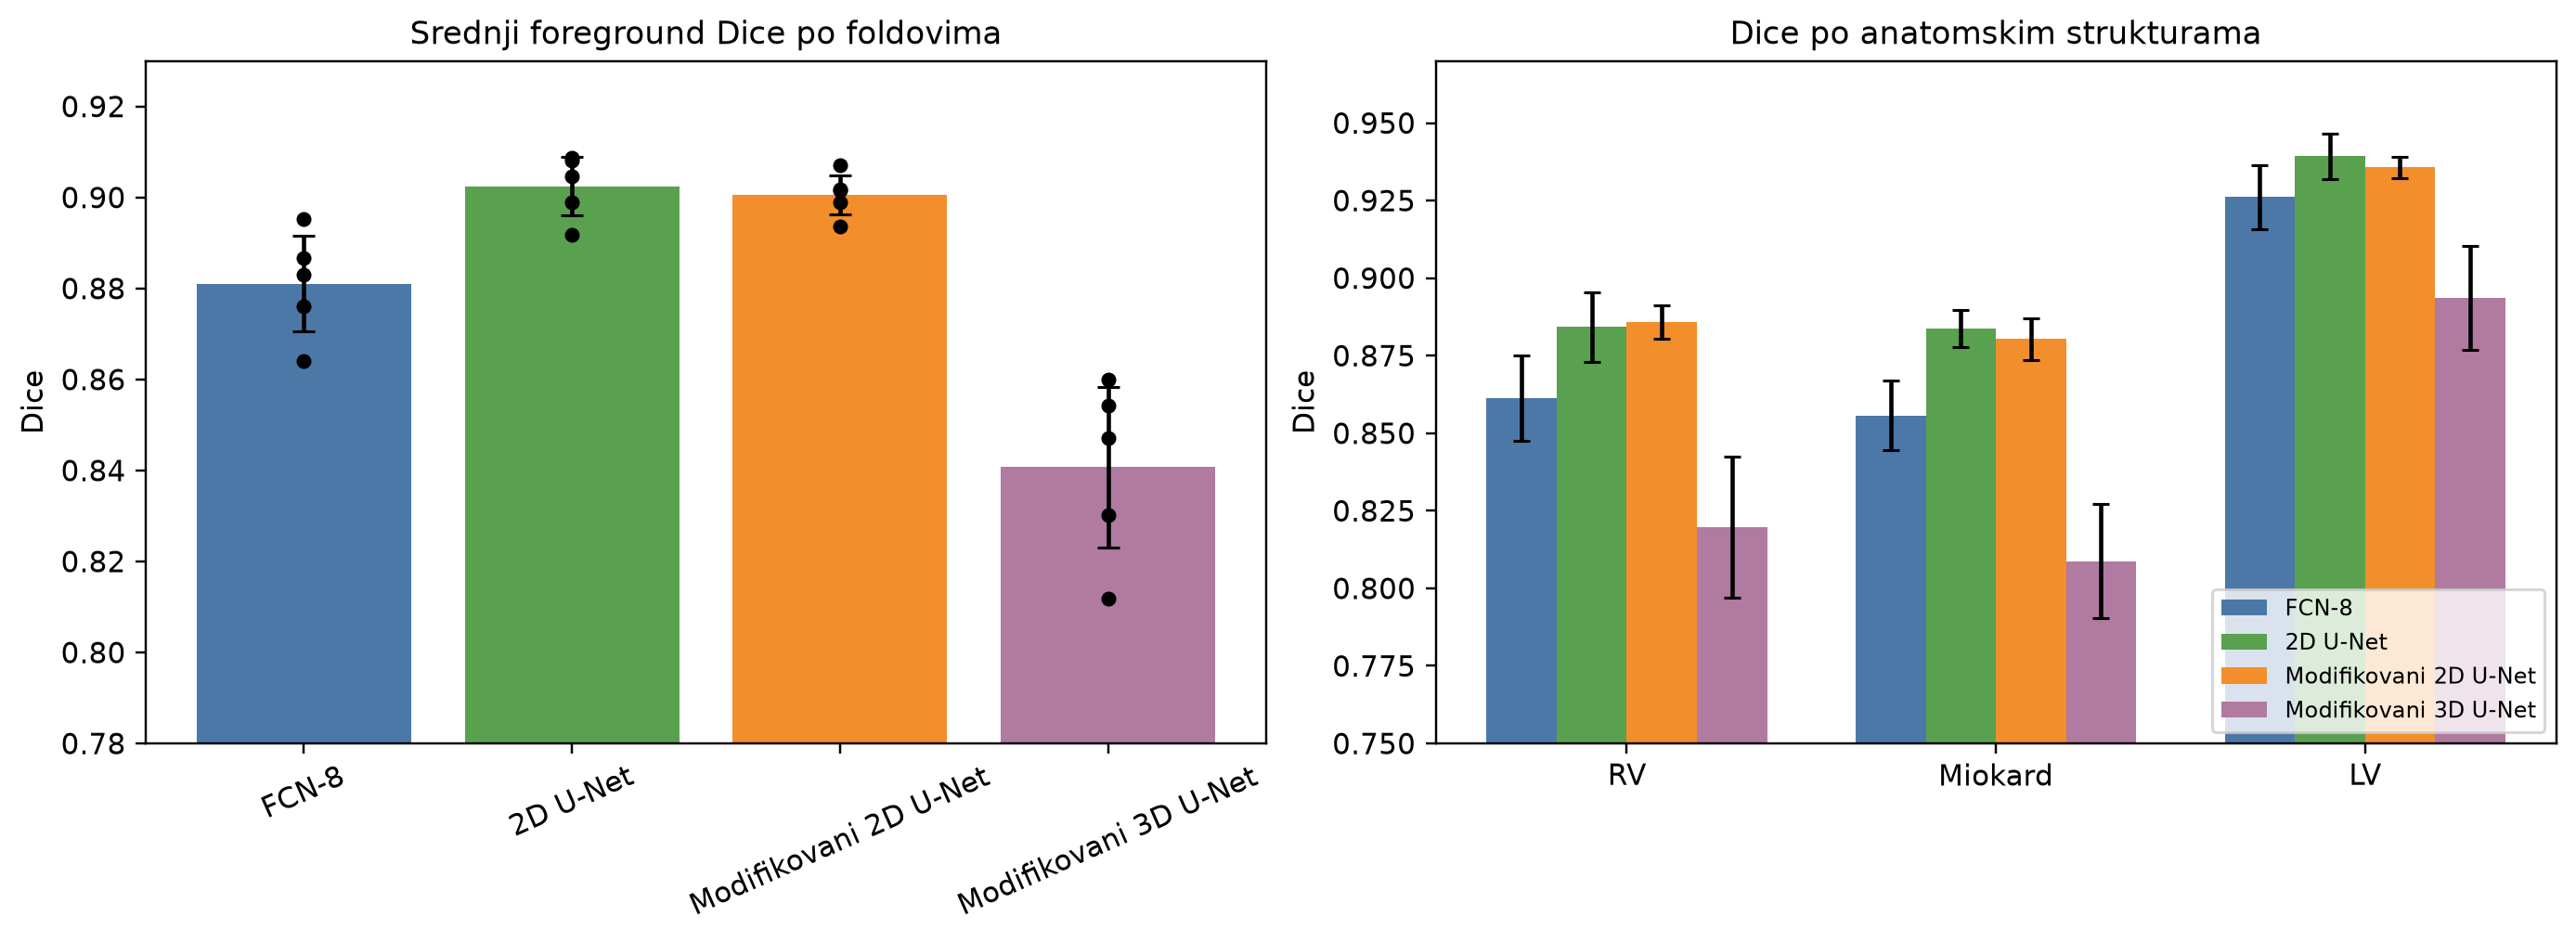
\includegraphics[width=\textwidth]{cv_model_comparison.png}
\caption{Poređenje modela: makro foreground Dice i Dice po strukturama. Tačke i trake greške prikazuju pet foldova.}
\label{fig:cv-models}
\end{figure}

\noindent Standardni 2D U-Net ima najbolji makro rezultat, ali je razlika u odnosu na modifikovani 2D U-Net mala: $0{,}0019$ Dice poena. Modifikovana arhitektura postiže najbolji RV Dice, uz približno 18,9\% manje parametara. LV je najlakša struktura za segmentaciju kod svih modela, dok su RV i miokard osetljiviji na nepravilnu geometriju, tanak zid i delimični volumenski efekat. Sličan obrazac prijavljen je i u izvornom radu \cite{baumgartner2017}.

\begin{table}[H]
\centering
\caption{Makro foreground Dice po validacionom foldu. Svaka vrednost nastaje iz 40 rekonstruisanih ED/ES volumena 20 validacionih pacijenata.}
\label{tab:cv-fold-dice}
\begin{tabular}{lrrrrr}
\toprule
Model & fold 0 & fold 1 & fold 2 & fold 3 & fold 4 \\
\midrule
FCN-8 & 0,8953 & 0,8640 & 0,8868 & 0,8760 & 0,8831 \\
2D U-Net & 0,9088 & 0,8918 & 0,9081 & 0,9047 & 0,8990 \\
mod. 2D U-Net & 0,8989 & 0,8937 & 0,9071 & 0,9016 & 0,9017 \\
mod. 3D U-Net & 0,8471 & 0,8302 & 0,8118 & 0,8601 & 0,8543 \\
\bottomrule
\end{tabular}
\end{table}

\subsubsection{FCN-8}
FCN-8 postiže CV Dice $0{,}8810\pm0{,}0105$, ASSD $0{,}9210\pm0{,}1699$ mm i HD $11{,}8831\pm1{,}1820$ mm. Najslabiji fold je fold 1 (Dice 0,8640), koji istovremeno ima najveći ASSD 1,1703 mm i HD 13,7664 mm. Po klasama, LV je najstabilnija struktura (Dice $0{,}9261\pm0{,}0103$), dok su RV i Myo na 0,8613 i 0,8557. Ansambl pet FCN-8 modela na 100 odvojenih volumena poboljšava Dice na 0,8934 i smanjuje HD na 10,5639 mm, ali zaostaje za obe 2D U-Net varijante.

\subsubsection{Standardni 2D U-Net}
Standardni 2D U-Net daje najbolji CV rezultat: Dice $0{,}9025\pm0{,}0064$, ASSD $0{,}7532\pm0{,}1108$ mm i HD $10{,}5616\pm0{,}7197$ mm. Dice je u svih pet foldova između 0,8918 i 0,9088, što pokazuje manju zavisnost od sastava validacionog podskupa nego kod FCN-8 i 3D modela. Ima najbolji LV rezultat (0,9393), a Myo Dice 0,8838 je praktično jednak RV rezultatu 0,8843. Na lokalno odvojenom skupu petomodelni ansambl zadržava prvo mesto: Dice 0,9109, ASSD 0,7613 mm i HD 9,8436 mm.

\subsubsection{Modifikovani 2D U-Net}
Suženi dekoder postiže CV Dice $0{,}9006\pm0{,}0043$, samo 0,0019 ispod standardnog 2D U-Net-a, uz najmanju varijabilnost između foldova. Najbolji je fold 2 sa Dice 0,9071, a raspon između najnižeg i najvišeg folda je 0,0134. Modifikovani model ima najbolji RV Dice (0,8858), dok su Myo i LV Dice 0,8803 i 0,9357. Petomodelni ansambl ostvaruje Dice 0,9085, ASSD 0,8096 mm i HD 9,8810 mm. Rezultat pokazuje da se približno petina parametara dekodera može ukloniti uz vrlo malu promenu preklapanja, uz skromno veće prosečne granične greške od standardnog modela.

\subsubsection{Anizotropni 3D U-Net}
Anizotropni 3D U-Net postiže CV Dice $0{,}8407\pm0{,}0176$, ASSD $1{,}8843\pm0{,}3567$ mm i HD $13{,}2831\pm0{,}8333$ mm. Najteži je fold 2, sa Dice 0,8118 i ASSD 2,5448 mm; to doprinosi najvećoj standardnoj devijaciji među upoređenim modelima. Po klasama su RV (0,8197) i Myo (0,8088) znatno slabiji od LV (0,8937), što ukazuje da dodatni kontekst kroz preseke ne nadoknađuje mali broj volumena i izraženu anizotropiju. Na test pacijentima ansambl poboljšava Dice na 0,8583 i ASSD na 1,4895 mm, ali i dalje ostaje iza 2D pristupa.

\subsection{Uticaj petostruke validacije}
Za razliku od jedne fiksne podele, pet foldova omogućava da svaki trening pacijent bude validacioni tačno jednom. Zato se uz srednju vrednost prijavljuje i standardna devijacija između foldova. Kod standardnog 2D U-Net-a makro Dice iznosi $0{,}9025\pm0{,}0064$ preko pet validacionih podskupova. Modifikovani 2D U-Net ima najmanju standardnu devijaciju Dice-a, $0{,}0043$, dok 3D U-Net pokazuje najveću, $0{,}0176$.

Raspodela ASSD i HD dodatno pokazuje zašto Dice sam nije dovoljan. Dva modela mogu imati slično preklapanje regiona, ali različitu najveću grešku granice. Kod 3D U-Net-a posebno se izdvaja jedan teži fold sa većim ASSD, što je u skladu sa osetljivošću volumetrijske obuke na mali broj uzoraka i mini-grupu veličine jedan.

\begin{figure}[H]
\centering
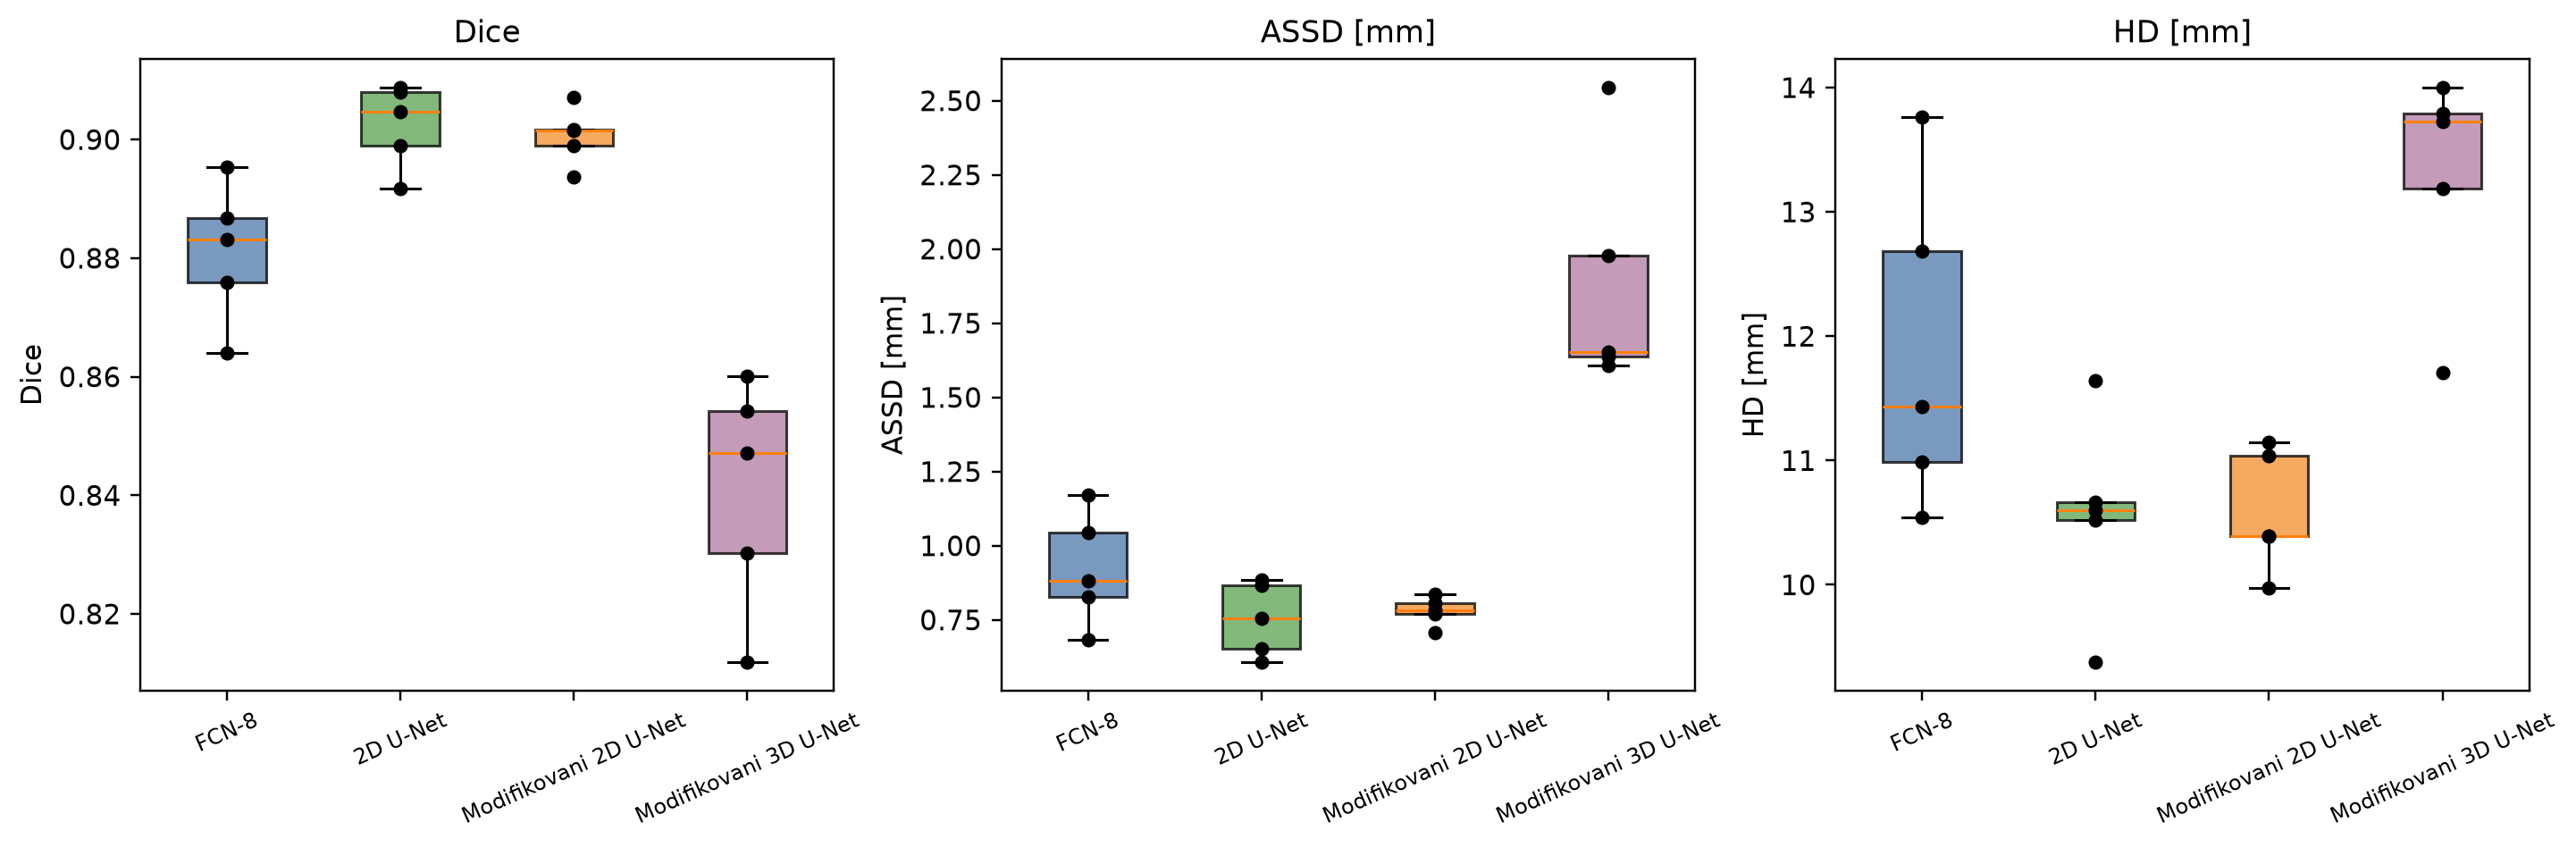
\includegraphics[width=\textwidth]{cv_fold_metric_spread.png}
\caption{Raspodela volumetrijskih metrika između pet foldova.}
\label{fig:cv-spread}
\end{figure}

\subsection{Završna evaluacija ansambla}
Za svaki model je pet fold modela iz epoha sa najboljim validacionim rezultatom objedinjeno prosekom softmax verovatnoća. Tabela~\ref{tab:test} prikazuje rezultat na 50 lokalno označenih test pacijenata, odnosno 100 ED/ES volumena. Standardni 2D U-Net zadržava prednost na odvojenom skupu. Ovi rezultati predstavljaju završnu lokalnu proveru.

\begin{table}[H]
\centering
\caption{Petomodelni ansambl na 100 odvojenih test volumena.}
\label{tab:test}
\begin{tabular}{lrrr}
\toprule
Model & Dice & ASSD [mm] & HD [mm] \\
\midrule
FCN-8 & 0,8934 & 0,8937 & 10,5639 \\
2D U-Net & \textbf{0,9109} & \textbf{0,7613} & \textbf{9,8436} \\
mod. 2D U-Net & 0,9085 & 0,8096 & 9,8810 \\
mod. 3D U-Net & 0,8583 & 1,4895 & 11,4728 \\
\bottomrule
\end{tabular}
\end{table}

\subsection{Krive učenja}
Sl.~\ref{fig:learning} prikazuje srednje vrednosti validacionog Dice koeficijenta po presecima i njegovu standardnu devijaciju kroz foldove. Krive služe za praćenje toka obuke. Najveći skokovi kod 3D mreže saglasni su sa malom mini-grupom i manjim brojem volumetrijskih uzoraka.

\begin{figure}[H]
\centering
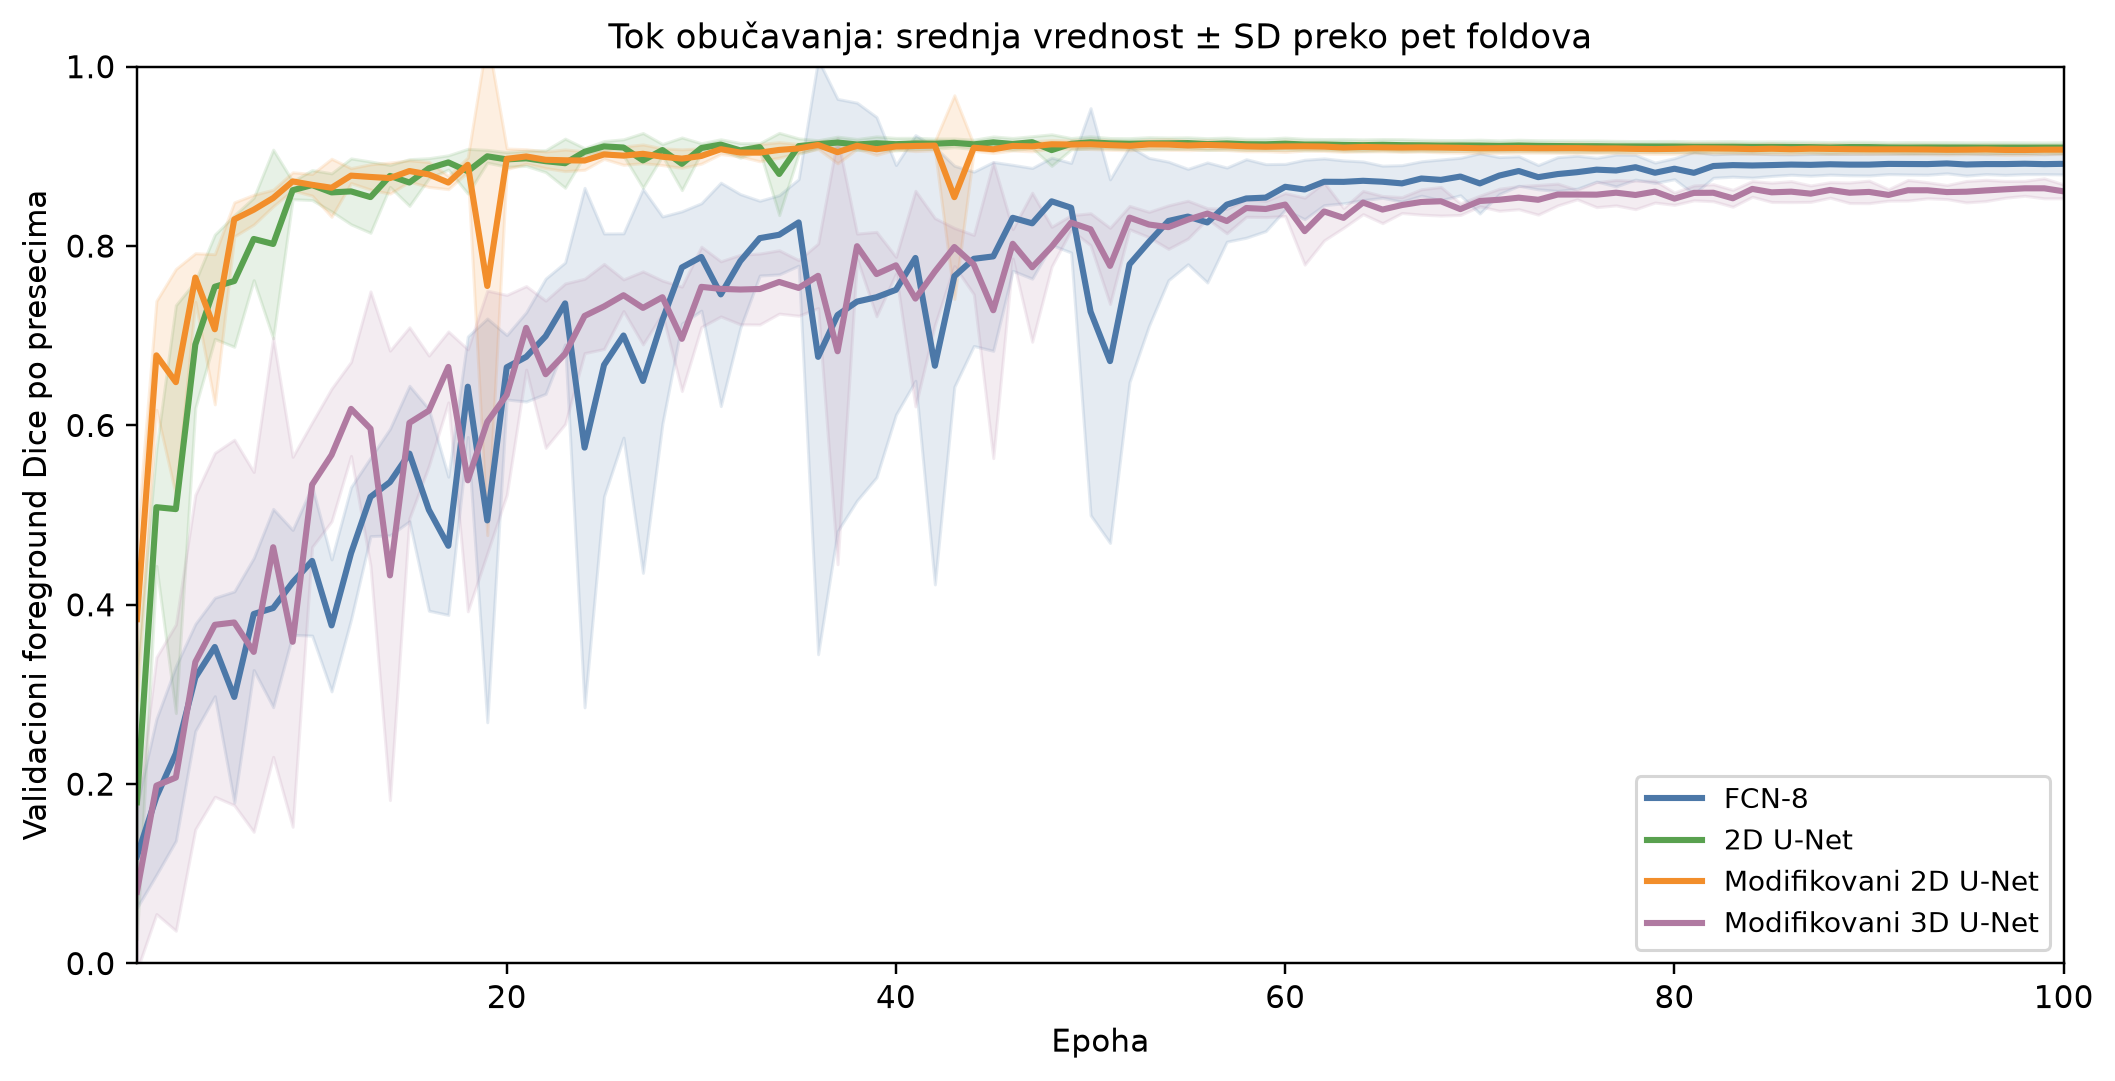
\includegraphics[width=0.96\textwidth]{cv_learning_curves.png}
\caption{Srednji validacioni foreground Dice po presecima tokom obuke.}
\label{fig:learning}
\end{figure}

\noindent Kod 2D modela validacioni Dice se ranije ujednačava nego kod 3D modela. Krive služe za izbor kontrolne tačke u svakom foldu, ali ne i za konačno poređenje arhitektura; za to se koriste rekonstruisani 3D volumeni iz Tabela~\ref{tab:cv-main} i \ref{tab:test}.

\subsection{Kvalitativna analiza predikcija}
Za poređenje svih arhitektura bira se po jedan unapred određen ED slučaj iz svakog validacionog folda: pacijenti 047, 051, 059, 052 i 055 za foldove 0--4. U svakom foldu bira se srednji pacijent po sortiranom identifikatoru, pa nijedan primer nije ručno izabran prema izgledu predikcije. Svaka mreža koristi samo težine odgovarajućeg folda, dakle nijedna nije učena na pacijentu prikazanom u svom redu. Zbog različite spacing-aware predobrade, preseci 2D i 3D modela nisu nužno na identičnom izvornom $Z$ položaju; za svaki prikaz bira se centralni presek sa najvećom površinom ekspertske foreground maske u reprezentaciji odgovarajućeg modela.

\IfFileExists{figures_cv/all_models_oof_prediction_comparison.png}{%
\begin{figure}[H]
\centering
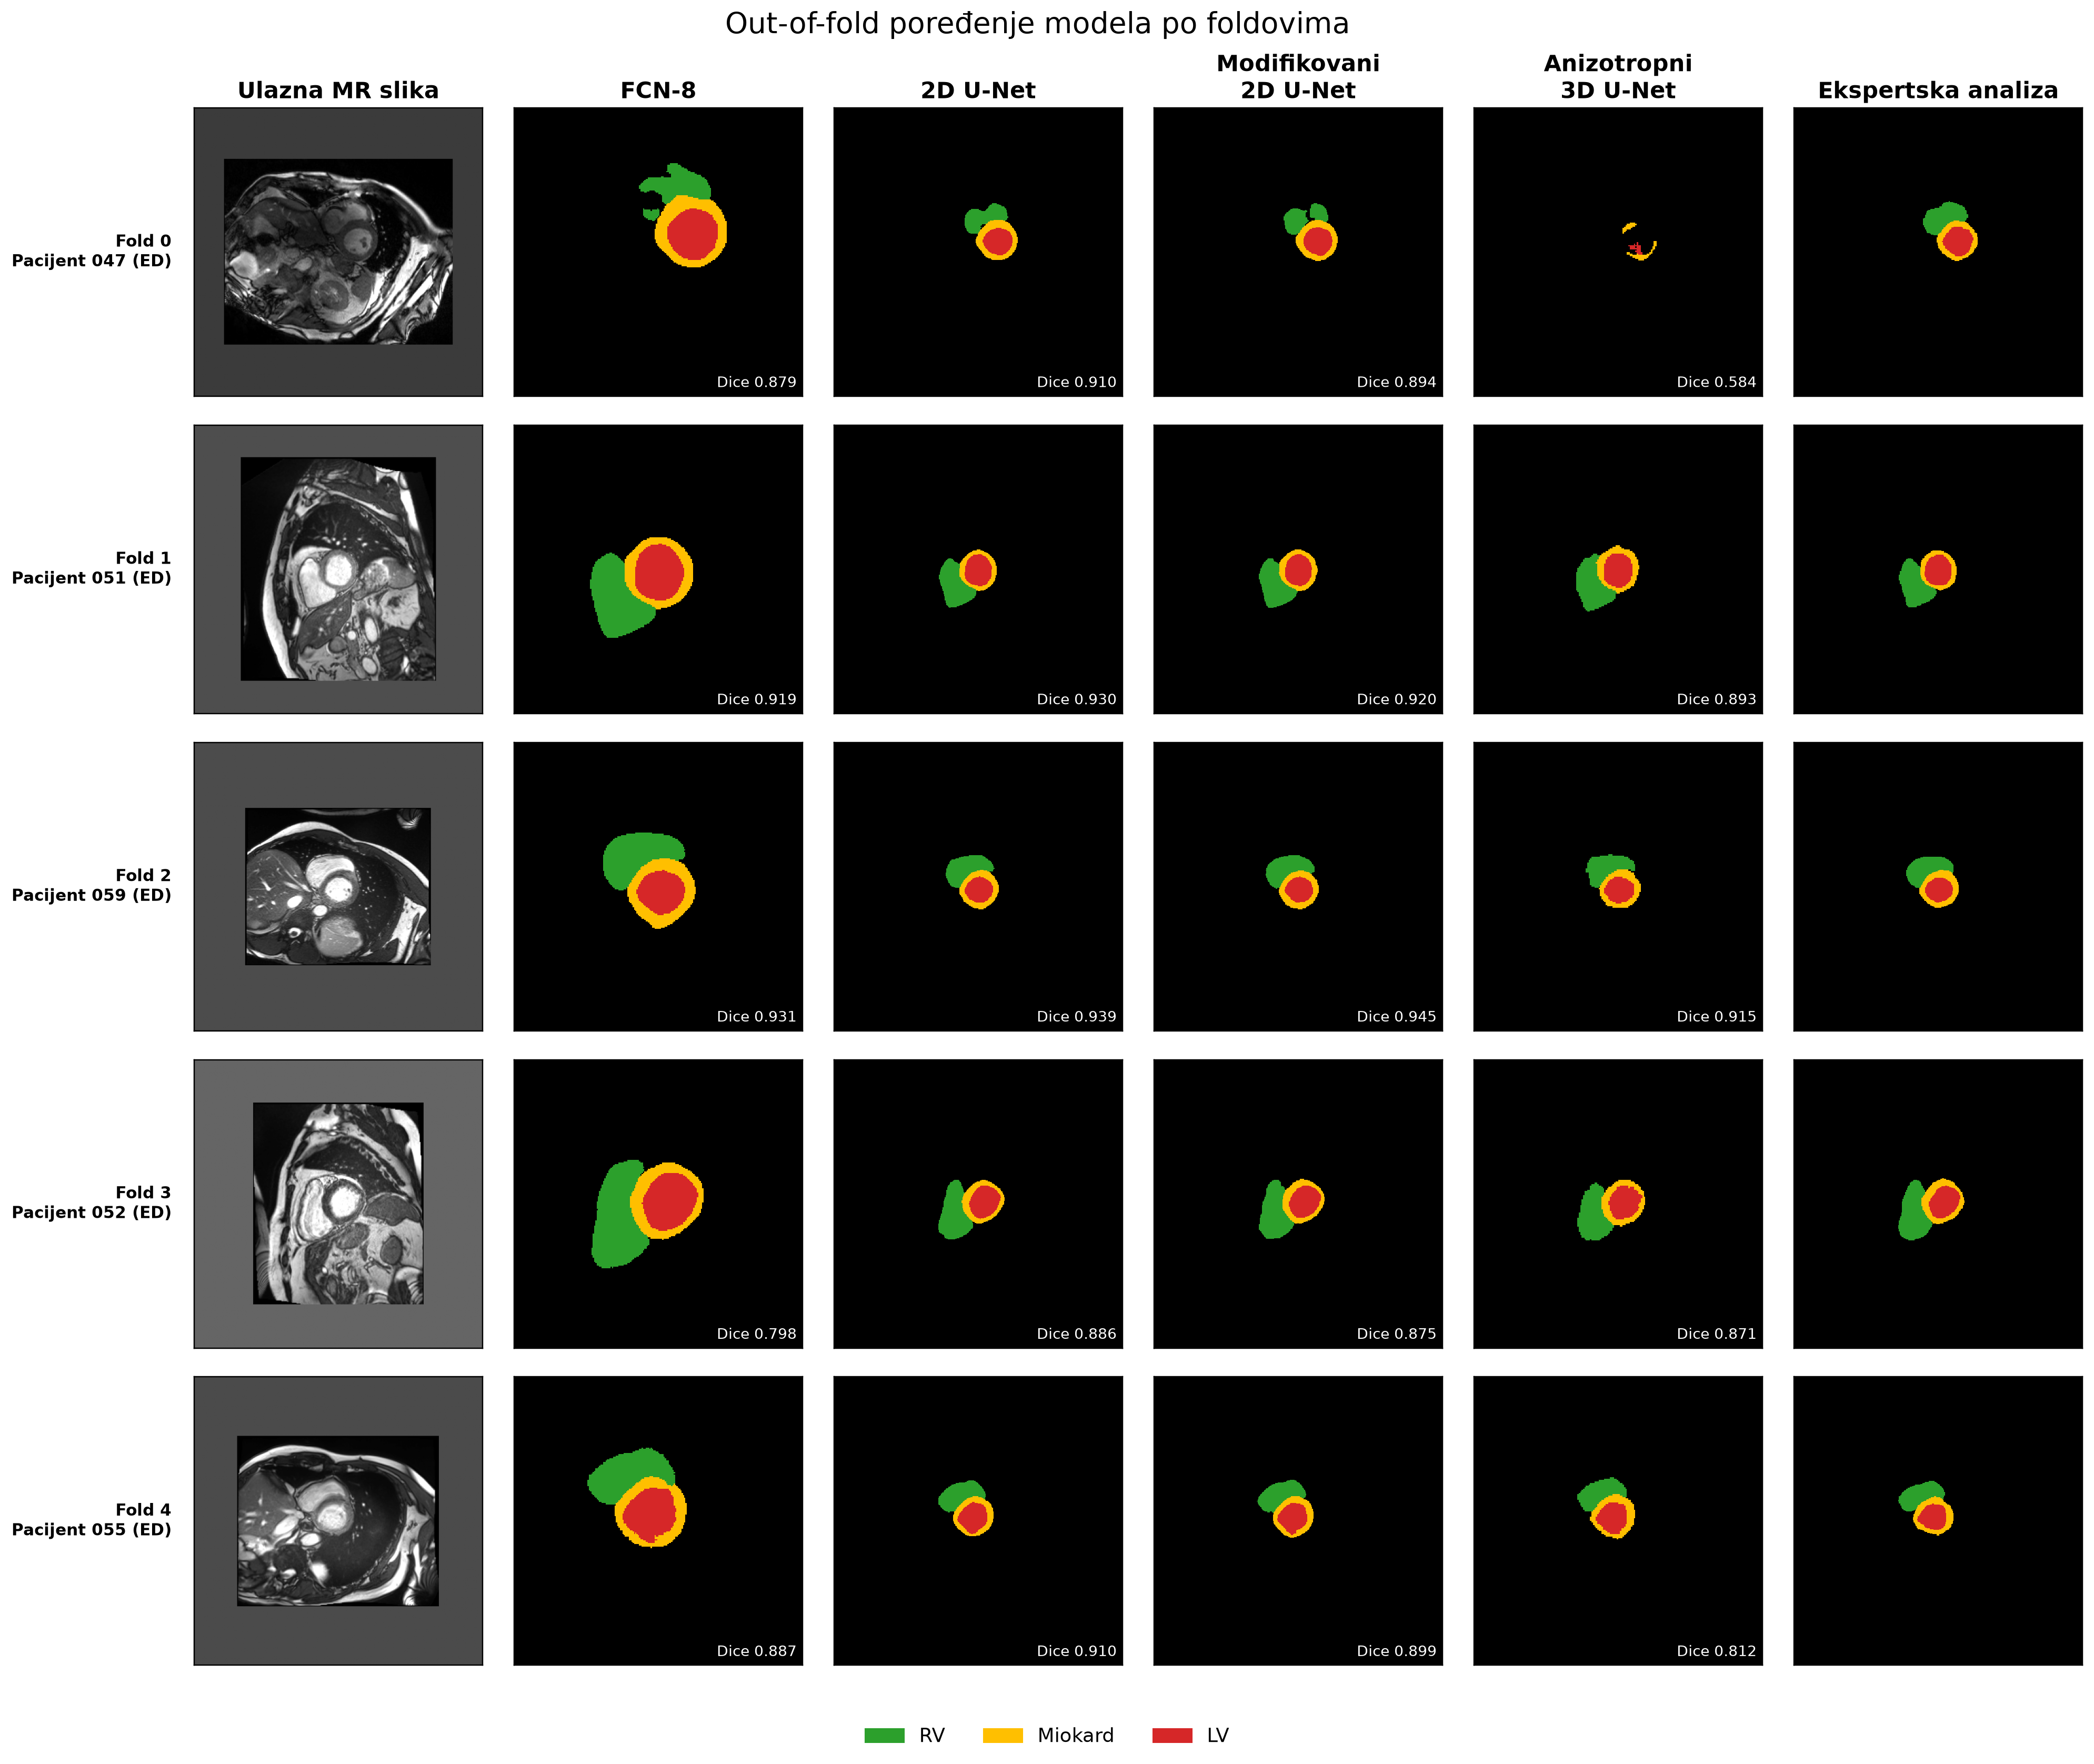
\includegraphics[width=0.94\textwidth]{all_models_oof_prediction_comparison.png}
\caption{Kvalitativno out-of-fold poređenje sva četiri modela na po jednom ED pacijentu iz svakog od pet foldova. Kolone predstavljaju ulaznu MR sliku, postprocesirane predikcije i ekspertsku masku; volumetrijski foreground Dice je naveden u svakoj predikcijskoj ćeliji.}
\label{fig:all-models-qualitative}
\end{figure}
}{%
\noindent\textit{Zajednički kvalitativni prikaz sva četiri modela generiše se na računaru sa težinama pomoću \texttt{scripts/visualize\_all\_models\_oof.py}. Skripta izvozi sliku i JSON sa checkpoint-ovima i Dice rezultatima, bez izmene izvornog teksta izveštaja.}\par
}

Kvalitativni prikaz dopunjuje volumetrijske tabele. Standardni 2D U-Net ima najveći Dice u foldovima 0, 1, 3 i 4 (0,910; 0,930; 0,886; 0,910), dok modifikovani 2D U-Net daje najbolji prikaz u foldu 2 (0,945). U obe 2D varijante konture LV i miokarda prate ekspertsku masku kroz svih pet primera, što vizuelno potvrđuje malu razliku njihovih prosečnih CV rezultata. FCN-8 je naročito slabiji na pacijentu 052 iz folda 3 (0,798), gde je vidljivo šire izdvajanje RV i miokarda u odnosu na referencu. Anizotropni 3D U-Net pokazuje najveću promenu između slučajeva: na pacijentu 047 dobija Dice 0,584 uz izrazito nepotpunu segmentaciju, dok na pacijentu 059 dostiže 0,915. Takva promenljivost je saglasna sa najvećom fold-level standardnom devijacijom ovog modela u Tabeli~\ref{tab:cv-main}. Posebnu pažnju treba obratiti na kontinuitet tankog miokarda, granice RV i male strukture pri vrhu i bazi, jer su upravo te oblasti najosetljivije na razlike između arhitektura i odgovaraju slabijim klasnim rezultatima.

\IfFileExists{figures_cv/unet2d_oof_prediction_comparison.png}{%
\begin{figure}[H]
\centering
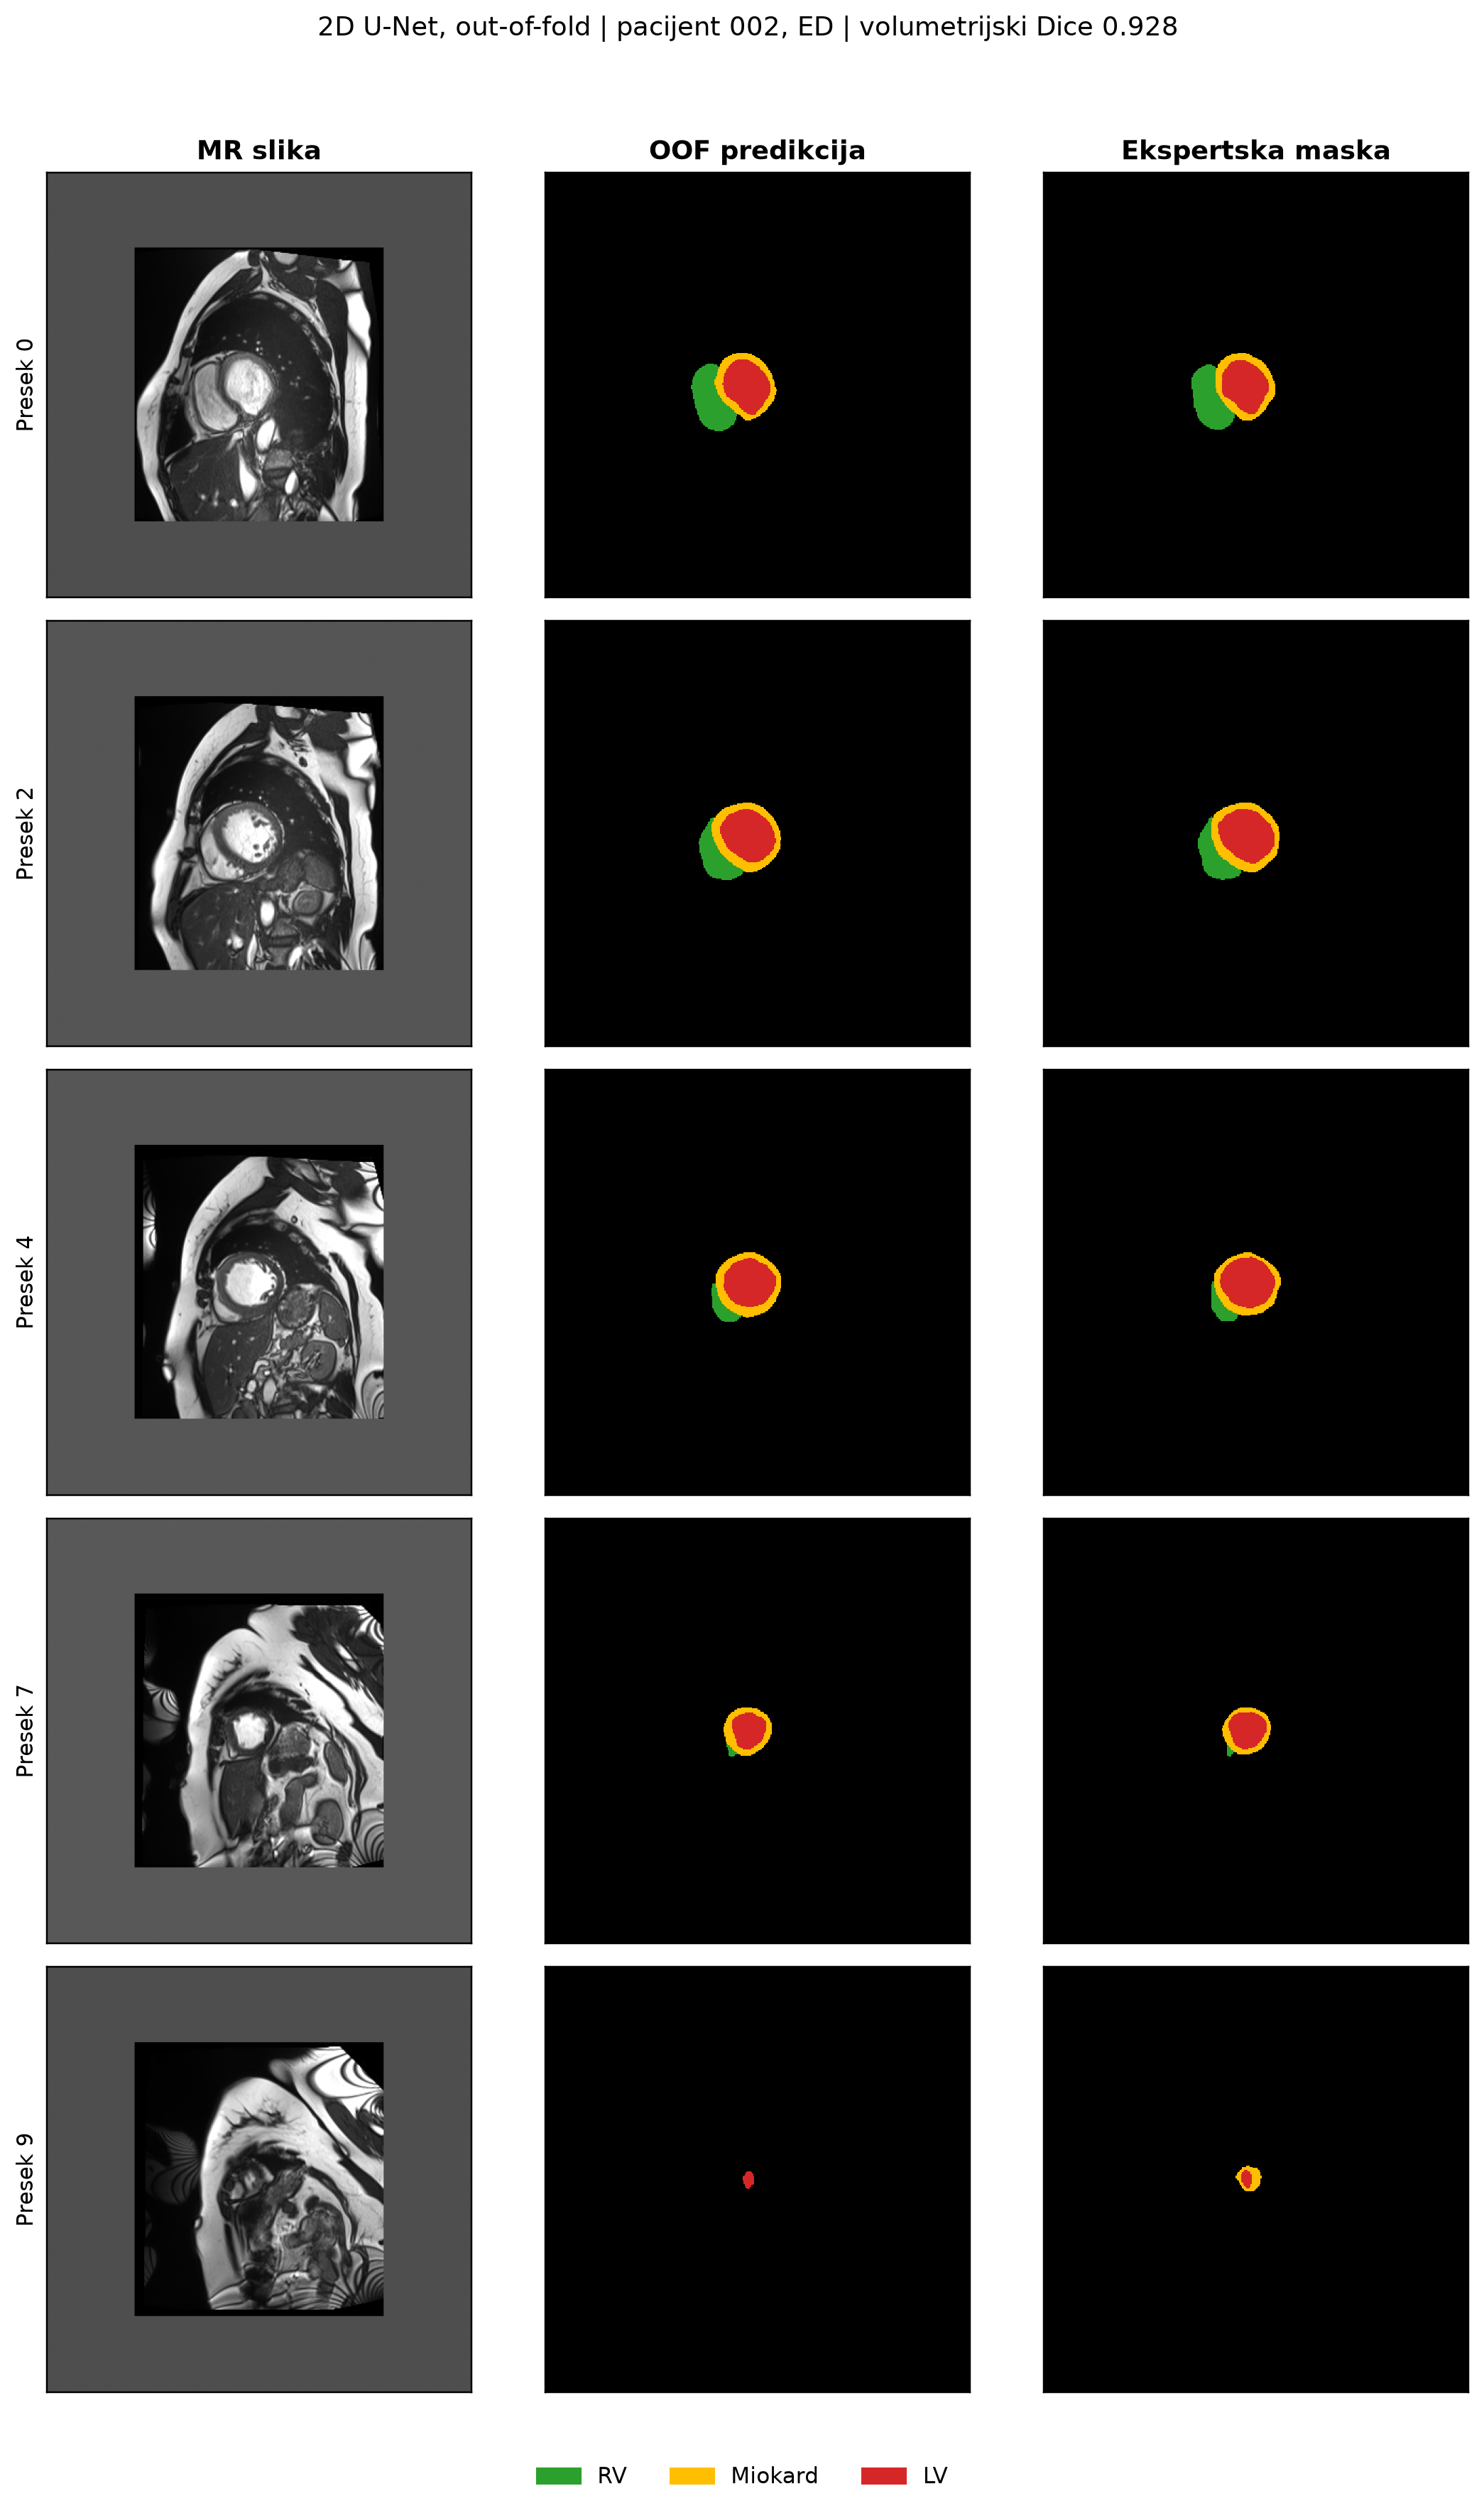
\includegraphics[height=0.80\textheight]{unet2d_oof_prediction_comparison.png}
\caption{Out-of-fold predikcije standardnog 2D U-Net-a i ekspertske maske kroz ED volumen pacijenta 002. Slučaj je deterministički izabran kao medijanski prema volumetrijskom foreground Dice-u među svim ED validacionim volumenima.}
\end{figure}
}{%
\noindent\textit{Kvalitativni out-of-fold prikaz generiše se na računaru koji poseduje pet najboljih kontrolnih snapshot-ova pomoću \texttt{scripts/visualize\_cv\_oof\_predictions.py}. U ovom radnom prostoru kontrolni snapshot-ovi nisu prisutni, pa se zastarela slika predikcija iz ranijeg eksperimenta ne koristi.}\par
}

Prikazani pacijent 002 pripada validacionom foldu 2 i predviđen je kontrolnim snapshot-om iz epohe 39; srednji volumetrijski foreground Dice iznosi 0,9276. Pošto model nije treniran na ovom pacijentu, prikaz je out-of-fold procena, a ne primer iz skupa za obuku. U centralnim presecima, gde su strukture velike i kontrastne, slaganje je veoma dobro. Veće razlike očekivano se javljaju pri bazi i vrhu, gde strukture zauzimaju mali broj piksela i brzo menjaju oblik između preseka. Miokard je posebno osetljiv, jer mala greška unutrašnje ili spoljne konture značajno menja preklapanje.

\subsection{Poređenje sa izvornim radom}
Poređenje sa Baumgartnerom i saradnicima u Tabeli~\ref{tab:paper} ima samo kontekstualni karakter. Objavljeni rezultati prosečavaju ED i ES protokolom koji nije identičan ovde korišćenoj predobradi, izboru hiperparametara i evaluaciji pune Hausdorffove udaljenosti. Ipak, odnos 2D i 3D pristupa ostaje sličan: 2D modeli dobro čuvaju detalje u ravni, dok 3D model plaća cenu anizotropije i većih memorijskih zahteva.

\begin{table}[H]
\centering
\caption{CV Dice ovog projekta i ED/ES prosek rezultata izvornog rada \cite{baumgartner2017}; poređenje je orijentaciono.}
\label{tab:paper}
\begin{tabular}{lrrr}
\toprule
Arhitektura & Ovaj projekat & Izvorni rad & Razlika \\
\midrule
FCN-8 & 0,881 & 0,902 & $-0,021$ \\
2D U-Net & 0,902 & 0,911 & $-0,009$ \\
modifikovani 2D U-Net & 0,901 & 0,914 & $-0,013$ \\
anizotropni 3D U-Net & 0,841 & 0,859 & $-0,018$ \\
\bottomrule
\end{tabular}
\end{table}

\subsection{Poređenje sa drugim ACDC takmičarima}
Organizatori ACDC izazova objavili su jedinstvenu evaluaciju deset pristiglih metoda na skrivenom test skupu od 50 pacijenata \cite{bernard2018}. Tabela~\ref{tab:contenders} sažima preostale takmičarske pristupe. Makro Dice u tabeli je naknadno izračunat kao neponderisani prosek šest objavljenih Dice vrednosti (LV, RV i Myo u ED i ES), dok je srednje HD rastojanje prosek odgovarajućih šest vrednosti u milimetrima. Nijedna od ove dve agregirane mere nije bila zvanična rang-metrika izazova.

\begin{table}[H]
\centering
\caption{Kontekstualno poređenje sa drugim ACDC takmičarima: zvanični skriveni test skup i izvedene agregirane mere \cite{bernard2018}; podebljan je lokalni rezultat ovog projekta.}
\label{tab:contenders}
\small
\begin{tabularx}{\textwidth}{Xrr}
\toprule
Metoda & Makro Dice & Srednje HD [mm] \\
\midrule
Isensee i sar. (ansambl 2D i anizotropnih 3D U-Net-ova) & 0,928 & 9,0 \\
Khened i sar. (gusti 2D U-Net) & 0,914 & 11,2 \\
Jang i sar. (2D M-Net) & 0,911 & 9,7 \\
Zotti i sar. (2D GridNet sa priorom oblika) & 0,911 & 9,6 \\
\textbf{Ovaj projekat (petomodelni ansambl standardnog 2D U-Net-a)} & \textbf{0,9109} & \textbf{9,8436} \\
Wolterink i sar. (2D dilatirana CNN) & 0,908 & 10,7 \\
Patravali, Jain i Chilamkurthy (2D U-Net) & 0,892 & 12,1 \\
Roh\'e, Sermesant i Pennec (višestruki atlas) & 0,892 & 12,1 \\
Tziritas i Grinias (nivoi skupova i MRF) & 0,836 & 15,8 \\
\bottomrule
\end{tabularx}
\end{table}

Najbolji takmičarski rezultat postiže ansambl 2D i anizotropnih 3D U-Net-ova Isenseea i saradnika. Više 2D varijanti zauzima gornji deo tabele, što je saglasno sa nalazom ovog projekta da standardni 2D U-Net najbolje koristi izrazito anizotropne ACDC snimke. U svim metodama LV je uglavnom lakša struktura, dok su miokard i RV u ES zahtevniji zbog tankog zida, nepravilnijeg oblika i manjeg preseka.

Petomodelni ansambl standardnog 2D U-Net-a ovog projekta ostvaruje Dice 0,9109 i HD 9,8436 mm na lokalno označenih 50 pacijenata 101--150. Te vrednosti su brojčano bliske grupi jakih originalnih 2D pristupa, ali se ne smeju tumačiti kao plasman na tabeli: takmičari su ocenjeni zvaničnim slepim evaluatorom na skrivenom test skupu, dok su ovde reference dostupne lokalno, a predobrada, postobrada i agregiranje metrika nisu nužno identični. Zato tabela služi za metodološki kontekst, ne za zvanično rangiranje.

\subsection{Ograničenja i mogućnosti unapređenja}
Petostruka validacija meri varijabilnost rezultata između podela, ali ograničen broj foldova i dalje ne predstavlja nezavisnu kliničku studiju. Dalji rad može obuhvatiti augmentaciju, kombinovane Dice--CE gubitke, 95-procentni HD, analizu neuspešnih slučajeva i izračunavanje kliničkih zapremina.

Posebno obećavajući pravac je transfer učenje. Umesto inicijalizacije svih težina slučajnim vrednostima, enkoder 2D mreže može se preuzeti iz prethodno obučene konvolucione mreže, a zatim dotrenirati za segmentaciju srca. Takav postupak obično ubrzava konvergenciju i može poboljšati prepoznavanje ivica i tekstura, naročito kada je broj označenih snimaka ograničen. Potrebno je prilagoditi prvi sloj jednokanalnom MR ulazu, a pri dotreniravanju koristiti manji korak učenja za prethodno obučene slojeve i veći za novu dekodersku i klasifikacionu glavu.

Transformerski modeli predstavljaju drugu moguću nadogradnju. Za razliku od konvolucija koje lokalno obrađuju ograničeno susedstvo, mehanizam pažnje može direktno povezati udaljene oblasti slike ili volumena i tako obezbediti širi prostorni kontekst. Hibridni CNN--transformer modeli, kao i segmentacione arhitekture zasnovane na prozorima pažnje, mogli bi da poboljšaju kontinuitet miokarda i razdvajanje RV od okolnih struktura. Njihovu veću računarsku složenost treba uravnotežiti hijerarhijskom pažnjom, manjim patch-evima i dotreniravanjem prethodno obučenih težina.

\section{ZAKLJUČAK}
Realizovan je spacing-aware postupak za automatsku višeklasnu segmentaciju srčanih struktura na ACDC cine-MR snimcima. Prostorni metapodaci sačuvani su tokom konverzije, 2D i 3D ulazi normalizovani su na fizičku skalu, a kvalitet je procenjen na rekonstruisanim volumenima sa rastojanjima u milimetrima.

Deterministička dijagnostički stratifikovana petostruka validacija omogućava procenu varijabilnosti rezultata između foldova. Standardni 2D U-Net postiže najveći srednji CV Dice, $0{,}9025\pm0{,}0064$, i najveći Dice petomodelnog ansambla na odvojenim test pacijentima, $0{,}9109$. Modifikovani 2D U-Net ostvaruje sličan rezultat uz manji broj parametara, dok anizotropni 3D U-Net u korišćenoj konfiguraciji ostvaruje slabiji rezultat.

Rezultati pokazuju da je za posmatrane anizotropne cine-MR volumene 2D segmentacija pogodnija od korišćene 3D varijante. Razmak kroz preseke je znatno veći od razmaka unutar ravni, pa susedni preseci nose manje pouzdanog lokalnog prostornog kontinuiteta nego susedni pikseli u ravni. 2D modeli zato uče iz većeg broja preseka, koriste ulaze više in-plane rezolucije i ne troše kapacitet na interpolisani kontekst kroz ravan. Nasuprot tome, 3D model obrađuje manje nezavisnih volumena, zahteva mini-grupu veličine jedan zbog većih aktivacija i osetljiviji je na promenu oblika struktura između udaljenih preseka. Anizotropne operacije ublažavaju ovaj problem, ali ga ne uklanjaju u potpunosti; to se vidi u nižem Dice-u i većoj varijabilnosti 3D rezultata.

Segmentacione maske imaju neposrednu kliničku vrednost, jer omogućavaju računanje zapremine LV i RV u ED i ES, a zatim udarnog volumena i ejekcione frakcije. Zapremina se dobija sabiranjem zapremine voksela unutar odgovarajuće komore, pri čemu se koriste stvarni prostorni razmaci. Iz LV miokardne maske može se izračunati i masa miokarda množenjem zapremine miokarda gustinom srčanog mišića. Zato greške segmentacije, posebno na granici miokarda i pri bazi i vrhu komora, ne utiču samo na Dice već se mogu preneti na izvedene kliničke pokazatelje.

Završni rezultat ansambla dodatno pokazuje korist kombinovanja pet modela. Svaki model je obučen na drugačijem skupu od 80 pacijenata i može napraviti različitu lokalnu grešku; prosečenje njihovih softmax verovatnoća smanjuje uticaj pojedinačne nestabilne predikcije pre konačnog izbora klase i postobrade. Kod standardnog 2D U-Net-a takav ansambl dostiže Dice 0,9109 na odvojenim pacijentima, u odnosu na prosečni CV Dice 0,9025 pojedinačnih fold-modela. Iako ove dve procene nisu strogo iste evaluacije, rezultat je saglasan sa očekivanjem da ansambl daje stabilniju i robusniju segmentaciju.

Zaključak ne znači da je 3D pristup načelno slabiji, već da izbor dimenzionalnosti mora pratiti fizičku rezoluciju snimanja, dostupni broj uzoraka i memorijski budžet. U scenariju sa gušćim presecima ili većim brojem volumena, 3D odnosno hibridni 2D--3D modeli mogli bi bolje iskoristiti međupresečni kontekst. Sačuvane podele, prostorni metapodaci i podešavanja eksperimenata omogućavaju ponavljanje postupka, proveru ovih pretpostavki i poređenje narednih arhitektura pod istim protokolom.

\clearpage
\section{LITERATURA}
\begin{thebibliography}{99}
\small
\bibitem{scmr2022} J. Schulz-Menger, D. A. Bluemke, J. Bremerich, et al., "Standardized image interpretation and post-processing in cardiovascular magnetic resonance -- 2020 update", \textit{Journal of Cardiovascular Magnetic Resonance}, vol. 22, art. 19, 2020; i SCMR smernice za izveštavanje CMR pregleda, 2022. \url{https://pmc.ncbi.nlm.nih.gov/articles/PMC9052489/}.
\bibitem{litjens2017} G. Litjens, T. Kooi, B. E. Bejnordi, et al., "A survey on deep learning in medical image analysis", \textit{Medical Image Analysis}, vol. 42, str. 60--88, 2017. DOI: \url{https://doi.org/10.1016/j.media.2017.07.005}.
\bibitem{baumgartner2017} C. F. Baumgartner, L. M. Koch, M. Pollefeys i E. Konukoglu, "An Exploration of 2D and 3D Deep Learning Techniques for Cardiac MR Image Segmentation", u \textit{STACOM 2017}, LNCS 10663, str. 111--119, 2018. \url{https://arxiv.org/abs/1709.04496}.
\bibitem{bernard2018} O. Bernard, A. Lalande, C. Zotti, F. Cervenansky, et al., "Deep Learning Techniques for Automatic MRI Cardiac Multi-structures Segmentation and Diagnosis: Is the Problem Solved?", \textit{IEEE Transactions on Medical Imaging}, vol. 37, no. 11, str. 2514--2525, 2018. DOI: \url{https://doi.org/10.1109/TMI.2018.2837502}.
\bibitem{acdcweb} CREATIS, "Automated Cardiac Diagnosis Challenge (ACDC)", zvanična stranica baze i izazova. \url{https://humanheart-project.creatis.insa-lyon.fr/database/#collection/637218c173e9f0047faa00fb}. Pristupljeno: septembar 2026.
\bibitem{long2015} J. Long, E. Shelhamer i T. Darrell, "Fully Convolutional Networks for Semantic Segmentation", u \textit{Proc. CVPR}, str. 3431--3440, 2015. \url{https://openaccess.thecvf.com/content_cvpr_2015/html/Long_Fully_Convolutional_Networks_2015_CVPR_paper.html}.
\bibitem{ronneberger2015} O. Ronneberger, P. Fischer i T. Brox, "U-Net: Convolutional Networks for Biomedical Image Segmentation", u \textit{MICCAI}, LNCS 9351, str. 234--241, 2015. DOI: \url{https://doi.org/10.1007/978-3-319-24574-4_28}.
\bibitem{cicek2016} Ö. Çiçek, A. Abdulkadir, S. S. Lienkamp, T. Brox i O. Ronneberger, "3D U-Net: Learning Dense Volumetric Segmentation from Sparse Annotation", u \textit{MICCAI}, LNCS 9901, str. 424--432, 2016. DOI: \url{https://doi.org/10.1007/978-3-319-46723-8_49}.
\bibitem{taha2015} A. A. Taha i A. Hanbury, "Metrics for evaluating 3D medical image segmentation: analysis, selection, and tool", \textit{BMC Medical Imaging}, vol. 15, art. 29, 2015. DOI: \url{https://doi.org/10.1186/s12880-015-0068-x}.
\end{thebibliography}
\end{document}
